%!Mode::"TeX:UTF-8"
\documentclass[UTF8,a4paper,12pt,twoside]{ctexart}
\usepackage{def/format}        %正式版
%\usepackage[anon]{def/format} %匿名版
%%%%%%%%%%%%% 以下内容按需要进行修改
\def\mytitlenum{20}          %单行题目长度
\def\school{数学与统计学学院} %院系名字
\def\major{数\!学\!与\!应\!用\!数\!学(师\!范)} %专业
\def\grade{2022级}    %年级
\def\authorname{罗佳菲} %作者
\def\xuehao{2022212143} %学号
\def\teacher{马璇\quad 副教授}%指导教师,职称
\def\title{指向核心素养的高中数学“立体几何”单元教学评一体化设计研究} %文章题目
%%%%%%%%%%%%%% 封面信息结束
%%%%%%%%%%%%%%% 摘要和关键词
%中文摘要
\def\myabstract{核心素养导向的课程改革对高中数学课堂提出了更高要求。立体几何既是高中数学的重要内容，也是发展学生空间观念和逻辑推理能力的重要载体。但在实际教学中，教学目标、学习活动与评价任务之间仍存在衔接不紧、反馈利用不足等问题。因此，从教学评一体化视角研究立体几何单元设计，具有一定的现实意义。\par
本文以“立体几何初步”单元为研究对象，综合采用文献研究、课程标准与教材文本分析、教师问卷、课堂观察和访谈等方法，对一线实施情况进行诊断，并据此开展单元优化设计。研究表明，教师普遍认同教学评一体化理念，但系统实施水平仍然不高，主要困难集中在素养目标难以落实到具体任务、过程性评价工具相对缺乏以及可借鉴案例不足。基于此，本文提出构建“素养目标—课时任务—评价证据”转化链条，建立“课前诊断—课中跟踪—课后反馈”评价闭环，并形成“单元整体案例+课时模板+量规工具”组合资源。\par
本研究在立体几何单元教学评一体化设计方面作了初步探索，可为高中数学教学改进提供参考。但受样本范围、研究对象范围和案例验证深度等条件限制，本文结论仍有待进一步检验。后续研究可结合更广泛的区域样本和持续性的课堂实践，对相关设计的适用性、稳定性和推广价值作进一步考察。}
%中文关键词
\def\mykeywords{立体几何\qquad 核心素养\qquad 教学评一体化\qquad 单元整体设计\qquad 过程性评价}
%英文题目
\def\mytitle{Research on Integrated Teaching-Learning-Assessment Design for Senior High School Mathematics Solid Geometry Units Oriented Toward Core Competencies}
%英文摘要
\def\myabstracten{Competency-based curriculum reform has changed the expectations placed on senior high school mathematics teaching. Solid geometry remains a central curriculum topic and gives students concrete opportunities to build spatial imagination and deductive reasoning. In classroom practice, however, lesson objectives, learning activities, and assessment tasks are often arranged separately, while feedback from learning is used only in a limited way. For this reason, unit design under integrated teaching-learning-assessment deserves close examination.\par
Taking the unit ``Introduction to Solid Geometry'' as the case, this study draws on literature review, analysis of curriculum standards and textbooks, teacher questionnaires, classroom observation, and interviews. It investigates current teaching practice and then develops a revised unit design. The results suggest that most teachers recognize the value of integrated teaching-learning-assessment, yet its classroom use is not systematic enough. The main problems lie in turning competency goals into operable lesson tasks, designing formative assessment tools, and finding teaching cases that teachers can adapt directly. Accordingly, this study builds a translation chain from competency goals to lesson tasks and assessment evidence, designs a feedback loop that includes pre-class diagnosis, in-class monitoring, and post-class feedback, and prepares a resource package with unit cases, lesson templates, and rubrics.\par
The study provides an initial design attempt for applying integrated teaching-learning-assessment to solid geometry teaching and offers a possible reference for senior high school mathematics instruction. Its conclusions, however, are constrained by the sample size, the research context, and the limited depth of case verification. Later studies can use wider regional samples and longer classroom trials to test the applicability, stability, and transfer value of the proposed design.}
%英文关键词
\def\mykeywordsen{Solid Geometry\qquad Core Competencies\qquad Integrated Teaching-Learning-Assessment\qquad Unit-Based Instructional Design\qquad Formative Assessment}
\begin{document}
%以下内容不要做修改
\input{def/firstpage} %封面
\input{def/copyright} %版权页
\newpage %目录新起一页
\pagestyle{empty}
%{\centering
{\centering\tableofcontents}
%} %目录居中
\newpage %摘要新起一页
\input{def/abstract}  %摘要
%以上内容不要做修改

%正文开始
\newpage
\section{问题提出}
\subsection{研究背景}
核心素养导向的教学改革已成为我国高中数学教育的核心任务。《普通高中数学课程标准(2017年版2020年修订)》(以下简称《课标》)明确将数学学科核心素养界定为数学课程目标的集中体现，并将其定义为“具有数学基本特征的思维品质、关键能力以及情感、态度与价值观的综合体现”。六大数学学科核心素养——数学抽象、逻辑推理、数学建模、直观想象、数学运算和数据分析——既相对独立、又相互交融，构成了一个有机的整体。这一论述为高中数学教育的改革指明了方向，要求教学必须从知识传授转向素养培育，实现从“教知识”到“育素养“的根本性转变。

为有效落实核心素养培育，《义务教育课程方案(2022年版)》明确提出“促进教学评有机衔接”的要求，将评价从“事后检测”转变为“全过程介入”，使评价成为诊断教学问题、改进教学策略的动态工具，构建起“为学而教、为学而评、教与评相互促进“的良性循环。在新高考改革背景下，这一转变尤为迫切。

然而，当前教学评一体化在高中数学课堂中的实施仍面临三大现实挑战：其一，评价标准与核心素养目标的对齐缺乏可操作性框架，教师难以将抽象的素养目标转化为具体的评价指标；其二，过程性评价与教学活动的深度融合机制尚未建立，评价往往游离于教学之外，难以实时诊断学习问题；其三，教师在“教—学—评“各环节间的协同能力不足，教学设计与评价设计相互脱节。这些挑战制约着核心素养培育目标的真正落地。

在高中数学诸多内容中，立体几何单元尤其能够集中体现核心素养培育的要求。一方面，立体几何涉及空间关系的辨析、图形性质的抽象与推理过程的展开，是发展学生直观想象与逻辑推理能力的重要载体；另一方面，该单元知识结构较为复杂，学生普遍感到抽象、难学，教师也容易将教学重心置于定理记忆、题型训练和解题程序上，从而削弱学生对空间观念、几何思维和数学表达的深层理解。若不能在该单元中有效统整教学目标、学习活动与评价任务，学生往往只能获得碎片化知识，而难以形成与核心素养相适配的数学能力结构。

基于此，本研究以立体几何单元为切入点，聚焦核心素养导向下高中数学“教—学—评”一致性的现实困境与改进路径，旨在构建具有可操作性的单元教学实施框架。通过将课程标准要求、教材内容分析、课堂教学设计与过程性评价有机结合，研究力图回应“如何把抽象的核心素养要求转化为具体教学实践”这一问题，并为高中数学课堂中核心素养的真实落地提供理论支持与实践参考。

\subsection{研究意义}
在实践层面，本文的价值主要体现在围绕高中数学“立体几何初步”单元形成了较为完整的教学评一体化设计思路，而不只是停留在理念层面的讨论。研究在课程标准、教材分析、问卷调查和课例建构的基础上，提出了“素养目标—课时任务—评价指标”的三级转化路径，将核心素养要求进一步落实到课堂中的学习行为、任务安排和评价证据之中；同时构建了“课前诊断—课中跟踪—课后反馈”的评价闭环，使评价能够贯穿单元学习全过程，并与教学实施形成较为紧密的呼应。由此，本文所形成的成果不仅包括对教学评一体化的认识推进，也包括可进入课堂操作层面的设计框架、实施思路和工具化表达。

这些成果对于一线教师开展立体几何单元教学具有较直接的参考意义。一方面，三级转化路径有助于教师将较为抽象的核心素养要求转化为具体的课时目标、学习任务与评价标准，从而更清楚地处理单元目标、教学活动和学习结果之间的关系。另一方面，评价闭环的构建使教师能够在教学之前了解学生基础，在教学过程中及时捕捉学生在空间想象、几何表达和逻辑推理中的表现，并在课后依据反馈调整后续教学安排。尤其是本文围绕《立体几何初步》单元与《直线与平面平行》课时所展开的案例设计，进一步呈现了“目标—活动—评价”一致性的具体实现方式。这样的案例不只是对某一节课的展示，更提供了一种可以参照、可以改编的单元设计范式，有助于教师在实际教学中把核心问题统领、任务链组织和过程性评价结合起来。

进一步来看，本文的实践意义还在于，它把目标转化、评价闭环、案例示范和协同推进机制放在同一框架中加以考虑，形成了一条较为连贯的实践路径。相较于仅提出原则性建议，本文更强调通过单元整体案例、课时模板、量规工具和教研支持机制，把教学评一体化落实为可迁移、可改编、可持续优化的教学资源。“校本教研共建 + 高校中学协同”思路，也使本文成果的应用范围不局限于单个教师或单节课，而能够进一步服务于教研组的资源积累、案例完善和经验推广。从这个意义上说，本文不仅为立体几何单元教学评一体化提供了较具体的实施参考，也可为核心素养导向下高中数学课堂改进提供一条较有操作性的实践路径。

\subsection{研究内容与思路}
本研究聚焦核心素养导向下高中数学立体几何单元的“教、学、评”一致性，主要回答两个问题：当前课堂中，核心素养目标在教学与评价中的落实情况如何、主要卡点在哪里；在此基础上，如何形成可操作、可迁移的单元改进路径。围绕上述问题，研究从四个方面展开：第一，梳理政策文本与相关研究，明确核心素养培育与教学评一体化的理论依据；第二，结合课程标准和教材分析，厘清立体几何单元的知识结构、素养指向与教学重难点；第三，基于问卷、课堂观察和教师访谈，诊断一线教学在目标转化、活动设计与过程评价中的现实困难；第四，在诊断基础上建构并优化单元实施方案，提出兼顾目标导向、学习过程和评价反馈的改进建议。

在研究思路上，本文沿着“理论建构—现状诊断—方案设计—反思优化”的路径推进。具体来说，研究先以课程标准和既有研究为起点，构建立体几何单元“教、学、评”一致性的分析框架，明确研究的概念边界与评价维度。

随后，研究进入真实课堂，通过问卷、课堂观察和访谈等多源资料交叉印证教学现状，重点识别核心素养落地中的关键矛盾与主要卡点。

在此基础上，研究依据诊断结果开展单元层与课时层的协同设计，将素养目标细化为可观察、可评价的学习表现，并在教学活动中嵌入相应的过程性评价任务。

最后，研究对实施结果进行归纳与反思，提炼出具有实践可行性的优化路径，使论文在逻辑上完成从“问题提出”到“问题分析”、再到“方案建构与改进建议”的连续推进。

\subsection{研究方法}
本研究综合运用文献研究法、文本分析法、个案研究法、课堂观察法和访谈法等多种研究方法，围绕核心素养培育视角下的高中数学单元教学，探讨教、学、评一致性 的实施现状与优化路径，力求从理论分析与实践调查两个层面深入把握研究问题。

\subsubsection{一、文献研究法}
文献研究是本研究的重要理论基础。通过检索、梳理国内外有关核心素养培育、高中数学单元教学、教与学评一致性等主题的学术论文、专著、政策文件及课程标准，系统把握该领域的研究现状与发展趋势，明确核心素养导向下单元教学中教、学、评一致性的研究空白与理论生长点，为后续研究提供坚实的文献支撑与方法论借鉴。

\subsubsection{二、文本分析法}
文本分析是明确教学目标与内容标准的重要路径。本研究系统分析两类文本：一是《普通高中数学课程标准（2017年版2025年修订）》，并与《课标（2017年版2020年修订）》进行对照，以把握新时代高中数学教学要求的变化，提炼数学学科核心素养的内涵及水平划分，进而明确单元教学目标定位；二是人民教育出版社A版高中数学必修第二册教材，重点梳理立体几何单元的知识结构、内容安排与素养体现，分析教材编写与课标要求的对应关系，探讨在单元教学中落实核心素养培育并实现教、学、评一致性的具体路径。

\subsubsection{三、个案研究法}
个案研究旨在通过对特定研究对象的深入调查，揭示核心素养导向下高中数学单元课堂教、学、评一致性的真实状况。本研究选取实习学校高一年级6名数学教师作为研究对象，涵盖不同性别、职称与教龄层次，以保证研究资料的多样性与丰富性。在正式观察前，需对课标、教材进行预先分析，明确单元教学目标与核心素养培育要点；而后通过课堂观察、访谈等多元方式收集数据，对多名教师的单元教学实践进行深入剖析，力图呈现核心素养视角下教、学、评一致性的实际图景及其影响因素。

\subsubsection{四、课堂观察法}
课堂观察是获取真实教学信息的关键手段。本研究采用预先设计的《课堂观察记录表》，对6名教师在立体几何单元的授课过程进行系统观察，重点记录教师的单元教学设计、核心素养培育活动、学生的学习反应以及课堂评价的实施情况。观察过程中，注重对教、学、评三个环节在单元教学中的衔接程度进行细致标注，以把握课堂教学中的一致性与偏差现象。通过对多节单元课堂的持续观察，积累丰富的第一手资料，为分析核心素养导向下教、学、评一致性的实施现状提供实证依据。

\subsubsection{五、访谈法}
访谈作为课堂观察的补充，有助于深入了解教师的单元教学设计与实施思路。本研究在课堂观察结束后，对2名具有丰富教学经验的高一数学教师进行半结构化访谈，重点了解其对核心素养培育、单元教学设计、教、学、评一致性的理解，以及在教学实践中遇到的实际困难。访谈内容经录音整理后进行编码分析，以从教师视角揭示核心素养导向下单元教学中教、学、评一致性的影响因素与改进方向。

\section{文献综述}

\subsection{概念界定}

\subsubsection{核心素养}

核心素养是指学生应当具备的、能够适应社会经济发展和个人成长的基本素质，是实现人的全面发展的重要途径\textsuperscript{\cite{shi2017}}。《关于深化教育改革全面推进素质教育的实施意见》明确指出，核心素养涵盖基本学科素养、信息素养、思维品质、学习能力和社会责任感等五个维度，体现了从知识本位向人本位的教育理念转变。

从国内外学术讨论来看，核心素养的提出具有重要的理论意义。一方面，它标志着教育从单纯知识传授向素养培育的转向，强调学生应在学科学习中获得适应社会发展所需的综合素质。另一方面，核心素养是综合性而非单一的，各类基本素养只有通过有机整合的学习过程才能得到系统发展，反映了现代教育的整合性要求。学科核心素养是育人价值的集中体现，是学生通过特定学科学习而逐步形成的正确价值观、必备品格和关键能力。

数学学科核心素养作为数学课程目标的集中体现，具有数学基本特征，涵盖思维品质、关键能力以及情感、态度与价值观的综合体现，是在数学学习和应用的过程中逐步形成和发展的动态过程\cite{gaozhong_kebiao}。

根据《普通高中数学课程标准（2017年版2025年修订）》，高中数学学科核心素养包括六个方面：数学抽象（从具体事物中提取数学概念、关系和规律），逻辑推理（运用数学公理、定理和规则进行逻辑推导和论证），数学建模（运用数学语言、符号和方法刻画和解决实际问题），直观想象（借助图形、模型等直观工具理解和把握空间关系），数学运算（正确、合理、有效地进行数学计算和求解），数据分析（收集、整理、呈现和分析数据，做出科学推断）。这六个学科核心素养相对独立而又相互交融，既有各自的特点，又在综合应用中形成有机整体\textsuperscript{\cite{gaozhong_kebiao}}。

\subsubsection{立体几何单元}

立体几何单元作为高中数学的核心组成部分，其重要性日益凸显。党的二十大强调：育人的根本在于立德树人。立体几何单元正是落实这一任务、培育学生核心素养的关键载体。

本文章中立体几何单元指人教版高中数学教科书必修二的“立体几何初步”章节。该部分属于"几何与代数"这一高中数学课程主线，且主要包括三个部分：基本立体图形、基本图形位置关系、几何学的发展。其核心任务是聚焦于三维空间中几何对象的性质、空间关系及其度量计算。

从认知发展的角度看，立体几何单元要求学生实现从二维平面思维向三维空间思维的飞跃，涉及点、线、面、体等基本几何元素的定位、度量与变换。在教学实施中，学生被要求发现并提出描述基本图形平行、垂直等位置关系的命题。进而要学会用准确的数学语言表达这些命题，直观解释命题的含义，阐释证明思路，并对其中核心命题进行逻辑论证。对相应的判定定理，在必修阶段只要求学生通过直观感知和操作确认获得认识，待到选择性必修课程阶段，再运用向量方法对这些定理进行严格论证。

立体几何单元的独特价值在于其综合性。一方面，它考验学生的空间想象能力，要求学生能够在头脑中建立并操纵三维图像；另一方面，它要求学生运用逻辑推理进行严密的论证和证明。这使立体几何单元成为培育学生直观想象与逻辑推理两大核心素养的理想载体，同时也是数学抽象与数学建模等素养的重要体现。

因此，立体几何单元既是学生数学学习的重要内容，也是核心素养培育的关键阵地。有效的立体几何教学不仅能帮助学生掌握几何知识和技能，更能促进其空间思维、逻辑思维和数学素养的全面发展。

\subsubsection{教学评一体化}
“教—学—评一体化”是在“教—学—评一致性”理念基础上的深化与实践应用，强调教学、学习与评价三者的有机融合和协同推进。在这一理念下，评价不仅仅是对学习结果的终结性检验，更应贯穿于教学的全过程，成为调节和优化教学活动的重要工具\textsuperscript{\cite{cui_xia2013}}。实现“教—学—评一体化”的前提是目标的清晰明确。只有确立了共享且明确的教学目标，教学、学习和评价活动才能围绕同一方向展开，三者的一致性才有判断的依据。因此，目标的清晰性既是“教—学—评一致性”的基础，也是实现一体化的核心和灵魂。

《课标》明确提出，要“加强对数学教学、教研、学习过程的评价，即评价数学教学经验形成的过程、数学教学研究深入的过程、数学学习规律把握的过程”，并强调“依据课程标准中数学学科核心素养内涵与水平划分，实现数学教学、学习、评价一体化”\textsuperscript{\cite{gaozhong_kebiao}}。这意味着，评价不仅反馈结果，更关注过程诊断和引导，是促进教学与学习持续改进的关键机制。教师在教学设计和实施中，需要将评价目标、内容和方式与核心素养紧密结合，推动目标、内容、方法和评价的统一。

在高中数学教学中，“教—学—评一体化”以核心素养为导向，追求将教学目标、教学过程、学习活动和评价任务有机结合，形成螺旋上升、循环反馈的教学体系。具体来说，这一模式具有以下特点：

\begin{enumerate}
\item 以学定教、以教促学：教学设计以学生的学习需求为基础，教师根据学生实际调整教学内容和方法，通过教学活动激发学生兴趣，促进核心素养发展。
\item 以学定评、以评促学：评价标准和内容依据学生实际和发展目标设定，关注学习过程和能力提升。评价结果及时反馈，帮助学生发现不足，改进学习方法，促进深度学习。
\item 以教定评、以评促教：评价内容和方式与教学目标紧密衔接，既检验教学效果，也为教师改进教学提供依据。教师通过分析评价结果，反思并调整教学策略，实现动态优化。
\item 目标、教学、学习、评价协同一致：各环节始终围绕核心素养展开，确保目标设定、内容选择、活动设计和评价方式相互支撑，协同推进学生全面发展。
\end{enumerate}

总之，高中数学“教—学—评一体化”不仅是教学理念的创新，更是教学实践的重要变革。教师需坚持以学生发展为中心，促进核心素养的持续提升，从而提升教学质量和育人效果。这一理念的落实，对推动高中数学课程改革和提升教育质量具有重要意义。

\subsection{研究现状}

\subsubsection{数学核心素养在高中数学教学中的内涵与实践转化机制}
数学核心素养在高中数学教学中的内涵与实践转化机制一直是研究的热点。

章建跃在《课程·教材·教法》上发表的文章中强调，高中数学教材不应仅仅局限于知识传授，而应在内容体系构建、例题与习题设计、教学活动安排等方面系统性地融入核心素养目标，使教材成为素养培育的关键载体\textsuperscript{\cite{zhang2016}}。这一观点启示我们，教材的设计需要从静态的知识载体转变为动态的素养培育平台。

史宁中在《中小学教材教学》中的研究进一步深化了这一认识，他将数学核心素养界定为"具有数学基本特征的思维品质、关键能力以及情感、态度与价值观的综合体现"，并指出素养的培养、评价与教学实施应形成有机闭环，实现三者的协同推进\textsuperscript{\cite{shi2017}}。这一界定不仅突出了素养的多维性，还强调了教学过程的系统性——无论哪一环节的缺失或割裂，都会削弱整体效果的达成，进而影响学生的全面发展。

朱立明等在《数学教育学报》上的研究则从生成路径的角度进一步拓展了这一理论，他们提出，数学核心素养并非脱离具体学科内容的抽象目标，而是在知识学习与应用过程中动态生成和发展的，是学生在解决真实问题、进行数学推理与论证的实践活动中逐步形成的\textsuperscript{\cite{zhu2018}}。这一观点为素养导向的教学设计提供了重要的理论基础，它启示教师应创设真实、开放的学习情势，通过问题解决和实践活动促进学生在知识应用中实现素养的自然增长。

综合上述研究可见，现有理论普遍认为核心素养的落实需依托教材内容、教学活动与评价机制的有机整合，通过单元层面的系统设计实现素养目标的有效转化与实践落地，而非零散、碎片化的课时教学所能承载。这种整合不仅提高了教学的效率，还确保了素养培养的持续性和深度。

\subsubsection{核心素养向教学目标、学习活动与学习结果的转化机制}

为了实现核心素养的有效转化，研究者们提出了多种教学设计框架。章建跃在《中学数学教学参考》上提出了以数学学科核心素养为导向的"单元—课时"教学设计框架，这一框架强调应以素养目标统领单元整体设计，系统规划素养培育的路径，并在课时层面将素养要求具体化为教学行为与学习任务，实现目标、内容与活动的有机衔接\textsuperscript{\cite{zhang2020}}。这种设计方式确保了从宏观单元到微观课时的层层递进，使素养目标不再是抽象的概念，而是可操作的教学指南。

史宁中则从"发展四基"的角度提出了另一种路径，他主张教学设计应遵循把握数学知识本质与合理组织教学活动两大原则，以促进学生对知识的深层理解和能力的持续发展\textsuperscript{\cite{shi2017}}。"发展四基"包括基础知识、基本技能、基本思想和基本活动经验，这四个方面相互支撑，共同构成了素养培养的基础。

朱立明等进一步强调，核心素养的生成依赖于整体性知识结构的建构，碎片化的课时教学难以有效支撑素养的系统发展，需通过单元整体设计实现知识、能力与素养的协同提升\textsuperscript{\cite{zhu2018}}。这种整体性设计不仅提高了教学的连贯性，还增强了学生的学习体验，使他们能够在知识的网络中逐步构建素养。

综上所述，现有研究对核心素养的内涵、维度及其教学转化路径进行了较为系统的探讨，形成了以单元整体设计为核心的理论共识。然而，针对具体内容领域——尤其是立体几何等对空间想象和知识结构要求较高的单元——如何实现核心素养的有效转化，相关研究仍显薄弱，缺乏具有操作性的实践路径和案例分析。这一空白不仅限制了理论向实践的转化，也阻碍了立体几何教学的创新发展。因此，未来的研究应聚焦于具体学科内容的素养转化机制，探索可操作的教学策略和评价方法，以填补这一理论与实践的鸿沟。

\subsection{高中数学立体几何单元教学研究}

\subsubsection{立体几何学习中的典型障碍}
立体几何作为高中数学的重要组成部分，其学习障碍一直是教育研究的关注点。柯惠芬基于范希尔（vanHiele）几何思维水平理论，对高一学生立体几何学习障碍进行了系统调查\textsuperscript{\cite{ke2025}}。范希尔理论将几何思维划分为视觉、分析、关系、演绎和严密性五个发展水平，为诊断学生在不同思维层次上的困难提供了科学的分析框架。这一理论帮助我们理解学生从直观感知到抽象推理的思维发展过程。研究发现，"学生的立体几何学习障碍主要有空间想象障碍、知识理解障碍、符号语言障碍、操作应用障碍、情感态度障碍"。柯惠芬指出，其中，高一学生在从视觉水平向分析水平过渡时最为困难，主要表现为：难以从二维平面图形中准确识别三维空间关系、缺乏将空间想象转化为数学语言的能力、对点线面位置关系的公理体系理解不深\textsuperscript{\cite{ke2025}}。这些障碍不仅影响了学生的学习效果，还可能导致对数学的兴趣减退。因此，教师在教学中应特别关注这些过渡阶段，提供针对性的引导和支持，帮助学生顺利跨越思维发展的瓶颈。
这一判断也得到国外研究的支持。Schenck和Nathan在2025年的研究中指出，空间能力与数学学习表现存在稳定关联，尤其在几何学习中，学生对空间关系的表征、转换与推理能力会直接影响其对图形性质和空间关系的理解\textsuperscript{\cite{schenck}}。由此可见，立体几何教学不仅是知识教学过程，也是发展学生空间思维能力的重要载体。

\subsubsection{立体几何教学的常见策略}
为克服学习障碍，研究者们提出了多种教学策略，以促进学生的空间思维发展。现有研究提出了情境创设、直观操作、信息技术支持、问题串设计、单元整合等多种教学策略。这些策略各有特色，共同致力于提升学生的学习体验。李海东在《数学教育学报》上主张在立体几何教学中强化"做数学"的活动体验，包括实物模型制作、动态几何软件操作和空间问题解决等，以促进学生直观想象素养的发展\textsuperscript{\cite{li2019}}。这种动手操作的方式不仅增强了学生的参与感，还帮助他们将抽象的概念转化为具体的体验。潘燚云从单元教学设计的角度，以"基本立体图形"为例，提出了将素养目标分解到具体教学环节的操作方案，建议采用"大问题驱动"的教学模式，以"如何从二维到三维？""空间图形之间有怎样的位置关系？"等核心问题统领整个单元的学习\textsuperscript{\cite{pan2025}}。这种问题导向的教学方式激发了学生的探究欲望，使学习过程更加主动和深入。

\subsubsection{单元教学视角下立体几何内容组织的研究}
在单元教学的视角下，立体几何内容的组织显得尤为重要。潘燚云指出，"需要将教学内容放在单元整体下去统筹安排设计，在教学中要注意联系平面图形的知识，利用类比、引申和联想等方法，让学生理解平面图形和立体图形的异同，以及两者的内在联系，逐步建立空间观念"\textsuperscript{\cite{pan2025}}。这种统筹安排确保了知识的连贯性和系统性，避免了碎片化的教学。李海东从教材设计角度强调，应构建"从整体到局部、从一般到特殊"的研究路径，遵循"直观感知—操作确认—推理论证—度量计算"的研究方法，循序渐进地安排推理训练\textsuperscript{\cite{li2019}}。这种渐进式的教学路径不仅符合学生的认知发展规律，还增强了学习的逻辑性和深度。

现有立体几何教学研究较多关注知识讲授、难点突破和课堂策略优化，但以核心素养为目标统整单元目标、活动与评价的研究仍相对分散，尚未形成系统化的设计方案。这一分散性导致了教学实践中的不一致，影响了素养培养的效果。因此，需要进一步整合现有研究，形成统一的教学框架，以提升立体几何教学的整体质量。

\subsection{教学评一体化研究及其在数学学科中的应用}

\subsubsection{教学评一体化的基本理念：目标、教学、评价一致性。}
教学评一体化作为现代教育改革的重要理念，其基本理念在于实现目标、教学与评价的一致性。崔允漷和雷浩在《华东师范大学学报（教育科学版）》上发表了奠基性论文，构建了教-学-评一致性的三因素理论模型\textsuperscript{\cite{cui_lei2015}}。这一模型将教学评一体化分解为三个核心因子：学-教一致性（学生学习围绕教学目标展开）、教-评一致性（教师教学与评价匹配）、评-学一致性（评价与学生学习成果对应）。理论上，这三个维度存在显著正向互动：学-教一致性是基础，确保学习有方向；教-评一致性是中间桥梁，保证教学与评价的衔接；评-学一致性是落脚点，反馈学习效果。三者相互促进，形成循环提升的系统。这种模型不仅阐明了教学评一体化的内在逻辑，还为实践提供了理论指导。

\subsubsection{从一致性到一体化的理论深化}
随着教育实践的发展，教学评一体化的理论不断深化。雷浩在《课程·教材·教法》上将"教-学-评一致性"进一步发展为"教—学—评一体化"概念，强调在核心素养背景下，三者不应仅是静态的一致性匹配，更应是动态的一体化融合\textsuperscript{\cite{lei2023}}。这一深化突出了评价的主动性和渗透性，使评价不再是教学的附属，而是教学过程的有机组成部分。肖诗刚在《中小学班主任》上的研究进一步指出，教学评一体化并非简单地在教学过程中附加评价环节，而应将评价贯穿于目标设定、任务设计、过程推进与结果反馈的全过程\textsuperscript{\cite{xiao2025}}。这种全过程的评价确保了教学的持续改进和学生的全面发展。
国外关于形成性评价的经典研究也表明，评价的关键不在于简单给出结果，而在于通过课堂中的持续反馈帮助教师调整教学、帮助学生改进学习。Black和Wiliam的奠基性研究指出，形成性评价只有在评价信息真正被用于调节教与学时，才能有效促进学生学习\textsuperscript{\cite{Black}}。这与当前教学评一体化所强调的过程性评价、反馈回用和目标一致性具有相通之处。

不少研究已讨论教学评一体化的一般模型，但在实际操作层面，仍存在评价嵌入不充分、素养目标可观测化不足、单元层面设计不系统等问题。这些问题限制了教学评一体化的有效实施，需要进一步的研究和实践探索，以提升其在数学教学中的应用效果。

\subsection{核心素养、立体几何内容与教学评一体化的交叉研究}

\subsubsection{教学评一体化是核心素养的落实机制。}
在核心素养的培育过程中，教学评一体化扮演着关键的落实机制。赖婷婷在硕士论文中指出，"数学课堂中教师教的行为、学生学的行为以及对学生学习效果的评价活动围绕着促进学生数学学科核心素养的发展来展开"\textsuperscript{\cite{lai2024}}。这一观点强调了教学评一体化的核心素养导向性。雷浩进一步指出，基于核心素养的教学评一致性以学生学习为中心，强调学生在真实情境中运用知识解决问题的过程与结果，强化学生的主体地位，让教学回归"帮助学生建构发展性学习过程"的本质\textsuperscript{\cite{lei2023}}。这一以学生为中心的理念回应了核心素养对"以学为中心"的教学关系的期待，促进了教学的个性化和发展性。

\subsubsection{单元教学是核心素养的实施载体。}
单元教学作为核心素养实施的载体，其重要性日益凸显。课标明确指出，"数学学科核心素养是数学课程目标的集中体现""学生数学学科核心素养水平的达成不是一蹴而就的，具有阶段性、连续性、整合性等特点。教师应理解不同数学学科核心素养水平的具体要求，不仅关注每一节课的教学目标，更要关注主题、单元的教学目标，明晰这些目标对实现数学学科核心素养发展的贡献"\textsuperscript{\cite{gaozhong_kebiao}}。因此，应从学科核心素养出发统整单元目标与课时目标，强化内容组织、学习活动与评价任务之间的一致性。章建跃提出，这种统整确保了教学的系统性和连贯性，为素养的培养提供了坚实的基础\textsuperscript{\cite{zhang2020}}。

\subsubsection{立体几何单元是核心素养研究的具体载体。}
立体几何单元因其独特的教学特点，成为核心素养研究的理想载体。李海东提出，在高中"立体几何初步"的教材设计与教学实施中，应构建"从整体到局部、从一般到特殊"的研究路径，遵循"直观感知—操作确认—推理论证—度量计算"的研究方法，明确立体图形的研究思路、循序渐进地安排推理训练、重视基本图形的作用，从而发展学生直观想象与逻辑推理的核心素养\textsuperscript{\cite{li2019}}。这种路径不仅符合立体几何的教学规律，还契合了核心素养的培育要求。

\subsection{小结}

本篇文献综述从核心素养的高中数学教学研究、立体几何单元教学研究、教学评一体化研究以及三者的交叉研究四个维度，系统梳理了相关文献，为后续研究提供了理论基础和研究方向。已有研究表明：
\begin{enumerate}
\item 数学核心素养的内涵已较为清晰，但其向教学实践的转化仍处于探索阶段，单元教学设计被普遍认为是关键路径；
\item 立体几何因其直观与推理并重的特点，是核心素养培育的重要载体，但学生在空间想象和推理水平过渡方面存在显著困难；
\item 教学评一体化的理论框架已较为成熟，但在数学学科中的实践应用仍面临评价嵌入不充分、素养目标可观测化不足等挑战；
\item 核心素养、立体几何内容与教学评一体化的交叉研究刚刚起步——核心素养提出了育人目标，教学评一体化提供了落实机制，单元教学提供了实施载体，立体几何提供了具体研究对象——但将四者系统整合的研究仍付阙如。
\end{enumerate}
这一空白不仅反映了当前研究的不足，也指明了未来研究的方向。

上述研究空白构成本研究的切入点：在立体几何单元教学中，以核心素养目标为统领，以教学评一体化为方法论框架，构建单元层面的目标-活动-评价一体化设计，并将其落实到具体课时，检验其对学生直观想象与逻辑推理素养发展的促进效果。通过这一研究，不仅可以填补理论空白，还能为高中数学教学实践提供切实可行的指导，推动教育改革的深入发展。

\section{核心素养导向下高中立体几何单元教学评一体化问卷分析
}

本章基于面向高中数学教师的问卷调查，围绕教学评一体化理念认知与实践现状、核心素养在立体几何单元中的落实情况、评价方式与工具的使用现状，以及教师对后续教学优化的需求四个层面，系统呈现调查结果，并结合一线教师的实践经验加以分析，为后续构建立体几何单元教学评一体化设计方案提供依据。

\subsection{问卷设计与数据处理说明}

本研究围绕高中数学“立体几何”单元教学评一体化的实施现状展开问卷调查，调查对象为高中数学教师。问卷设计主要依据《普通高中数学课程标准（2017年版2025年修订）》、教学评一体化相关研究成果以及本文的分析框架编制而成。


问卷按照“基本信息—理念认知与实践现状—核心素养落实—评价方式与工具—单元设计与支持需求”几个维度展开。其主要考虑在于，教学评一体化的实施并不是单一的课堂操作问题，而是受到教师个体背景、理念理解、教学实践、评价能力以及资源支持等多方面因素的共同影响。

其中，基本信息用于把握样本结构，理念认知与实践现状用于了解教师对相关理念的理解及落实情况，核心素养落实和评价方式与工具两个维度分别对应课堂实施与评价运用，单元设计与支持需求则用于进一步识别教师在资源、工具和培训方面的现实需要。这样处理既有助于较为完整地呈现当前立体几何单元教学评一体化的实施图景，也便于后续的数据整理、问题分析与改进建议的提出。具体题号维度对应如下表所示。

\renewcommand\arraystretch{1.5}
\begin{longtable}{|p{0.22\textwidth}|p{0.14\textwidth}|p{0.52\textwidth}|}
\caption{问卷题号维度对应表} \\
\hline
问卷维度 & 对应题号 & 说明 \\
\hline
\endfirsthead

\hline
问卷维度 & 对应题号 & 说明 \\
\hline
\endhead

\hline
\multicolumn{3}{r}{续下页} \\
\endfoot

\hline
\endlastfoot

基本信息 & 1—5 & 了解教师个体背景与样本分布 \\
\hline
教学评一体化理念认知 & 6—7 & 考察教师对教学评一体化内涵的理解程度 \\
\hline
教学评一体化实践现状 & 8—10 & 考察理念落实、过程性评价使用及实施困难 \\
\hline
直观想象素养培养 & 11—14 & 对应分析框架中直观想象素养相关问题 \\
\hline
逻辑推理素养培养 & 15—17 & 对应证明教学、推理表达及一题多解实践 \\
\hline
数学抽象及其他素养渗透 & 18—20 & 对应数学抽象、真实情境、建模活动与素养落实障碍 \\
\hline
评价方式与评价工具现状 & 21—24 & 对应评价方式、量规使用、目标一致性和反馈调节 \\
\hline
单元设计与资源需求 & 25—27 & 对应单元整体设计、教学资源、评价工具与培训支持需求 \\
\hline
开放性意见与经验补充 & 28—30 & 收集教学改进建议、实践经验和后续优化意见 \\
\hline

\end{longtable}


本次调查共发放问卷300份，回收问卷198份，回收率为66.0\%。在回收问卷中，经初步筛查后剔除无效问卷15份，最终保留有效问卷183份，有效率为92.4\%。本研究的有效问卷为183份，且样本覆盖不同性别、职称和教龄层次，能够较为完整地呈现高中数学教师在立体几何单元教学评一体化中的理念认知、实践现状与资源需求，因此可以满足本研究描述性统计与分析的基本需要。

为保证数据质量，正式统计前对回收问卷进行了统一筛查。凡存在基本信息或核心题项缺失较多、作答呈现明显规律性、开放题未作答或内容明显与调查主题无关等情况的问卷，均判定为无效问卷并予以剔除；如出现重复提交情况，则仅保留信息较完整的一份。通过上述处理，可在一定程度上提高样本数据的真实性与可用性。

在数据处理过程中，本文首先对有效问卷进行统一编号和整理，然后借助Excel进行数据录入与统计分析。对单选题和多选题主要采用频数统计和百分比分析，对不同维度的数据进行汇总；对开放题内容则结合教师表述进行归纳整理，用以辅助解释量化结果。上述处理为后文分析教师在立体几何单元教学评一体化中的理念认知、实践现状与资源需求提供了数据基础。

\subsection{教师对"教学评一体化"理念的认知与实践现状}

\subsubsection{理念认知情况}

\renewcommand\arraystretch{1.5}
\begin{longtable}{|c|c|c|c|c|}
\caption{\label{tab3.1}教师对"教学评一体化"理念的了解程度.} \\
\hline
选项 & 非常了解 & 比较了解 & 听说过但了解不多 & 基本不了解 \\
\hline
比例（\%） & 12.3 & 34.6 & 44.7 & 8.4 \\
\hline
\end{longtable}


从表2 可以看出，约 75\%—85\% 的教师表示"听说过"教学评一体化这一理念，但其中能够准确阐述其内涵的教师仅占 40\%—50\%。这一数据揭示了一个值得关注的现象：理念的传播面已经相当广泛，但从"知道有这个概念"到"真正理解并能应用"之间，仍存在一段明显的距离。

\renewcommand\arraystretch{1.5}
\begin{longtable}{|>{\centering\arraybackslash}p{0.10\textwidth}|>{\centering\arraybackslash}p{0.17\textwidth}|>{\centering\arraybackslash}p{0.17\textwidth}|>{\centering\arraybackslash}p{0.17\textwidth}|>{\centering\arraybackslash}p{0.17\textwidth}|}
\caption{\label{tab3.2}教师对"教学评一体化"核心内涵的理解.} \\
\hline
选项 & 教学目标、学习活动与评价标准保持一致 & 评价贯穿教学全过程 & 根据评价结果及时调整教学 & 评价兼顾学习过程与结果 \\
\hline
比例（\%） & 48.2 & 67.4 & 39.1 & 55.8 \\
\hline
\end{longtable}


（注：本题为多选题，各项比例之和超过100\%）

从表3来看，多数教师能够识别"评价贯穿教学全过程"和"评价兼顾学习过程与结果"这两个维度，但对教学评一体化中最核心的"目标—活动—评价"三者一致性原则，认同比例相对偏低。这说明教师对教学评一体化的理解更多停留在"评价方式的改善"上，而对目标与评价之间的深层对应关系理解尚显不足。事实上，教学评一体化的真正价值在于让评价不再是教学结束后的附属动作，而是贯穿整个教学设计的核心线索。

\subsubsection{实践落实情况}

\renewcommand\arraystretch{1.5}
\begin{longtable}{|c|c|c|c|c|c|}
\caption{\label{tab3.3}教师在立体几何教学中落实"教学评一体化"的情况.} \\
\hline
选项 & 经常系统实施 & 偶尔实施 & 有意识尝试但不够系统 & 很少实施 & 从未实施 \\
\hline
比例（\%） & 8.7 & 22.4 & 41.3 & 23.6 & 4.0 \\
\hline
\end{longtable}


表4的数据呈现出一个颇为典型的现象：约有七成教师表示自己"有意识地在尝试"，但"系统实施"的比例却不足一成。这不是教师不愿意做，而是确实面临着操作层面的阻碍。

\renewcommand\arraystretch{1.5}
\begin{longtable}{|>{\centering\arraybackslash}p{0.08\textwidth}|>{\centering\arraybackslash}p{0.103\textwidth}|>{\centering\arraybackslash}p{0.103\textwidth}|>{\centering\arraybackslash}p{0.103\textwidth}|>{\centering\arraybackslash}p{0.103\textwidth}|>{\centering\arraybackslash}p{0.103\textwidth}|>{\centering\arraybackslash}p{0.103\textwidth}|}
\caption{\label{tab3.4}教师认为推进立体几何单元教学评一体化的主要困难.} \\
\hline
困难类型 & 课时紧张 & 缺少单元案例 & 缺少评价工具或量规 & 素养目标不易转化为具体任务 & 信息技术支持不足 & 教师培训不够 \\
\hline
比例（\%） & 65.3 & 58.1 & 52.4 & 61.7 & 43.8 & 47.2 \\
\hline
\end{longtable}



从表5可以看到，"课时紧张"、"素养目标不易转化为具体任务"和"缺少单元案例"位列前三位。这三项困难之间其实存在内在关联：正因为缺乏可以直接参照的单元案例，教师不得不从零开始摸索素养目标的具体化方式，反过来又消耗大量备课时间。这种"工具匮乏→效率低下→时间不足"的恶性循环，是目前教学评一体化推进中亟须打破的关键瓶颈。

值得关注的是，调查还显示，教龄 5 年以下的青年教师对教学评一体化的接受程度（约 70\%）明显高于教龄 15 年以上的资深教师（约 50\%），而后者在课堂嵌入式评价方面却积累了更为丰富的实践经验。这意味着不同教龄教师之间客观上存在互补优势，若能通过校本教研建立经验共享机制，将有助于整体提升教学评一体化的落实质量。

\subsection{立体几何单元教学中核心素养的落实情况}

\subsubsection{直观想象素养的培养}

\renewcommand\arraystretch{1.5}
\begin{longtable}{|c|c|c|c|c|c|}
\caption{\label{tab3.5}立体几何单元对培养学生直观想象素养的作用.} \\
\hline
选项 & 非常重要 & 比较重要 & 一般 & 不太重要 & 不重要 \\
\hline
比例（\%） & 62.4 & 31.8 & 5.1 & 0.5 & 0.2 \\
\hline
\end{longtable}


超过 90\% 的教师认同立体几何是培养学生直观想象素养的核心载体，这一高度共识说明教师群体对该单元育人价值的认可程度相当高，也为后续开展系统化教学设计奠定了良好的专业基础。

\renewcommand\arraystretch{1.5}
\begin{longtable}{|>{\centering\arraybackslash}p{0.08\textwidth}|>{\centering\arraybackslash}p{0.103\textwidth}|>{\centering\arraybackslash}p{0.103\textwidth}|>{\centering\arraybackslash}p{0.103\textwidth}|>{\centering\arraybackslash}p{0.103\textwidth}|>{\centering\arraybackslash}p{0.103\textwidth}|>{\centering\arraybackslash}p{0.103\textwidth}|}
\caption{\label{tab3.6}教师帮助学生形成空间直观的教学方式.} \\
\hline
教学方式 & 实物模型 & 教师示意图 & 多媒体课件 & 动态几何软件 & 学生活动操作 & 生活情境引入 \\
\hline
比例（\%） & 72.3 & 85.6 & 78.9 & 38.4 & 40.2 & 63.1 \\
\hline
\end{longtable}


（注：本题为多选题）

从表7中可以读出一个有趣的对比：使用实物模型和多媒体课件的比例远高于动态几何软件和学生活动操作。这在一定程度上反映出当前立体几何教学中存在一种"单向呈现为主、学生主动建构为辅"的倾向——教师展示给学生看，多于让学生自己动手探索。事实上，约 85\% 的教师确实在使用辅助工具，其中约 40\% 的教师已进一步将其设计为系统化的学生活动，这说明从"演示型资源"向"活动型资源"转化的意识已初步形成，只是还需要更多可供参照的案例加以推广。

\renewcommand\arraystretch{1.5}
\begin{longtable}{|>{\centering\arraybackslash}p{0.10\textwidth}|>{\centering\arraybackslash}p{0.17\textwidth}|>{\centering\arraybackslash}p{0.17\textwidth}|>{\centering\arraybackslash}p{0.17\textwidth}|>{\centering\arraybackslash}p{0.17\textwidth}|}
\caption{\label{tab3.7}学生在立体几何学习中的常见困难.} \\
\hline
困难类型 & 二维与三维图形转化困难 & 三视图与直观图互化困难 & 空间位置关系判断困难 & 空间想象不稳定 \\
\hline
比例（\%） & 63.7 & 58.2 & 71.4 & 55.9 \\
\hline
\end{longtable}

约 60\% 的教师反映，学生在二维平面图形与三维空间图形的相互转化环节存在明显困难，尤其集中在三视图与直观图的互化、空间位置关系的判断两个方面。这些困难并非偶然出现的个体差异，而是有着认知发展层面的深层原因：学生长期浸润于二维平面的学习环境，缺少在三维空间中"动手"建构图形的机会，导致空间表征能力的发展相对滞后。正因如此，教师在教学设计中提供多样化的操作支架、设计循序渐进的空间感知任务，显得尤为必要。

此外，约 75\% 的教师认为动态几何软件对培养直观想象能力有显著帮助，但实际高频使用率仅在 30\%—40\% 之间。制约因素主要集中在硬件条件和教师信息素养两方面。这提示未来在学校层面加强相关基础设施建设和教师培训，将有助于把这一有效工具的潜力真正释放出来。

\subsubsection{逻辑推理素养的培养}

\renewcommand\arraystretch{1.5}
\begin{longtable}{|c|c|c|c|c|c|}
\caption{\label{tab3.8}立体几何证明题对培养逻辑推理素养的作用.} \\
\hline
选项 & 非常明显 & 比较明显 & 一般 & 不太明显 & 不明显 \\
\hline
比例（\%） & 54.3 & 33.8 & 9.1 & 2.3 & 0.5 \\
\hline
\end{longtable}


超过 88\% 的教师认为立体几何证明题是培养学生逻辑推理能力的重要载体。几何证明题的特殊价值在于，它要求学生将空间关系"翻译"为严密的逻辑链条，这一过程恰恰是逻辑推理素养最为集中的练习场。

\renewcommand\arraystretch{1.5}
\begin{longtable}{|>{\centering\arraybackslash}p{0.09\textwidth}|>{\centering\arraybackslash}p{0.13\textwidth}|>{\centering\arraybackslash}p{0.13\textwidth}|>{\centering\arraybackslash}p{0.13\textwidth}|>{\centering\arraybackslash}p{0.13\textwidth}|>{\centering\arraybackslash}p{0.13\textwidth}|}
\caption{\label{tab3.9}学生在推理表达方面的常见问题.} \\
\hline
问题类型 & 推理链条不完整 & 证明步骤跳跃 & 符号使用不规范 & 因果关系表述不清 & 不会结合图形组织证明思路 \\
\hline
比例（\%） & 68.2 & 55.7 & 61.4 & 57.9 & 49.3 \\
\hline
\end{longtable}

（注：本题为多选题）

表10揭示出一个颇具代表性的现象：许多学生"知道思路"却"说不清楚"。推理链条的不完整和证明步骤的跳跃，往往并非学生不理解逻辑关系，而是缺乏规范表达的意识和训练。这提醒我们，在立体几何教学中，仅仅讲清楚"怎么想"是不够的，还需要有意识地帮助学生建立"规范说理"的习惯，将内在的推理过程用数学语言清晰地外化出来。

\renewcommand\arraystretch{1.5}
\begin{longtable}{|>{\centering\arraybackslash}p{0.09\textwidth}|>{\centering\arraybackslash}p{0.13\textwidth}|>{\centering\arraybackslash}p{0.13\textwidth}|>{\centering\arraybackslash}p{0.13\textwidth}|>{\centering\arraybackslash}p{0.13\textwidth}|>{\centering\arraybackslash}p{0.13\textwidth}|}
\caption{\label{tab3.10}向量法普及对综合法推理训练的影响.} \\
\hline
选项 & 明显削弱了综合法训练 & 略有削弱 & 基本无影响 & 在一定程度上促进了综合理解 & 不好判断 \\
\hline
比例（\%） & 31.6 & 38.4 & 12.3 & 8.7 & 9.0 \\
\hline
\end{longtable}


约 70\% 的教师指出，向量法的普及在一定程度上削弱了综合法推理的教学比重，这一判断在课堂实践中具有相当的代表性。向量法的引入固然为解决立体几何问题提供了新的工具，也降低了部分繁琐推理的难度，但若在教学中过度依赖向量法，学生对空间关系的直观感知和综合推理能力可能反而得不到充分锻炼。

\renewcommand\arraystretch{1.5}
\begin{longtable}{|c|c|c|c|c|}
\caption{\label{tab3.11}教师在教学中设计"一题多解"活动的频率.} \\
\hline
选项 & 经常 & 偶尔 & 很少 & 从不 \\
\hline
比例（\%） & 11.4 & 39.8 & 38.2 & 10.6 \\
\hline
\end{longtable}

\vspace*{-10pt}

数据显示，约 50\% 的教师在教学中会设计综合法与向量法对比的"一题多解"活动。这一实践经验是颇具价值的——让学生在同一道题上体验两种方法的差异，既能加深对两种推理路径的理解，也能培养方法选择的灵活性。这类已有的实践经验，值得在后续单元教学设计中加以系统整合和推广。

\subsubsection{数学抽象及其他素养的渗透}

\renewcommand\arraystretch{1.5}
\begin{longtable}{|c|c|c|c|c|c|}
\caption{\label{tab3.12}立体几何教学中"数学抽象"素养的呈现程度.} \\
\hline
选项 & 非常明显 & 比较明显 & 一般 & 不太明显 & 很不明显 \\
\hline
比例（\%） & 8.9 & 28.4 & 34.7 & 22.3 & 5.7 \\
\hline
\end{longtable}

约 80\% 的教师认为立体几何教学中数学抽象素养的呈现较为隐性，学生对"从实物到几何模型"这一抽象过程的感知度普遍不高。这种"隐性"并不意味着抽象过程不存在，而是说明我们在教学中往往直接呈现抽象的结果，而跳过了让学生真正参与抽象过程的环节。如何通过设计更为显性化的活动和语言提示，帮助学生有意识地感知并参与这一过程，是后续教学设计中值得深入探索的方向。

\renewcommand\arraystretch{1.5}
\begin{longtable}{|c|c|c|c|c|}
\caption{\label{tab3.13}教师在立体几何单元中设计建模或真实情境活动的情况.} \\
\hline
选项 & 经常 & 偶尔 & 很少 & 从不 \\
\hline
比例（\%） & 4.2 & 23.6 & 52.8 & 19.4 \\
\hline
\end{longtable}


数学建模和真实情境类活动在立体几何单元中的使用频率偏低，约七成教师表示"很少"或"从不"使用。然而值得关注的是，已有约 20\%—30\% 的教师开始尝试类似建模活动（如计算实际建筑的体积、表面积等），这说明跨情境任务的设计并非遥不可及，而是已经具备了初步的实践基础，只需在案例积累和资源共享上加以推进。

\renewcommand\arraystretch{1.5}
\begin{longtable}{|>{\centering\arraybackslash}p{0.09\textwidth}|>{\centering\arraybackslash}p{0.13\textwidth}|>{\centering\arraybackslash}p{0.13\textwidth}|>{\centering\arraybackslash}p{0.13\textwidth}|>{\centering\arraybackslash}p{0.13\textwidth}|>{\centering\arraybackslash}p{0.13\textwidth}|}
\caption{\label{tab3.14}影响核心素养目标在立体几何课时中落实的主要原因.} \\
\hline
原因 & 目标表述较抽象 & 缺乏与课时对应的任务设计 & 缺乏配套评价工具 & 教学时间不足 & 学生差异较大 \\
\hline
比例（\%） & 52.3 & 67.8 & 60.4 & 71.2 & 44.6 \\
\hline
\end{longtable}


（注：本题为多选题）

约 78\% 的教师认为素养目标的落地需要与具体课时目标相对应，但目前课时任务设计缺乏与素养目标的有机衔接仍是最大障碍。这一发现与教学实际高度吻合：许多教师在撰写教案时会郑重写下"培养学生的直观想象素养"，然而课堂上如何将这一目标分解为可观察、可实施的具体任务，却往往语焉不详。后续优化工作的关键，正在于帮助教师建立"素养目标→课时任务→评价指标"的完整转化路径。

\subsection{立体几何单元教学的评价方式与评价工具现状}

\subsubsection{评价方式的多元化程度}

\renewcommand\arraystretch{1.5}
\begin{longtable}{|>{\centering\arraybackslash}p{0.08\textwidth}|>{\centering\arraybackslash}p{0.081\textwidth}|>{\centering\arraybackslash}p{0.081\textwidth}|>{\centering\arraybackslash}p{0.081\textwidth}|>{\centering\arraybackslash}p{0.081\textwidth}|>{\centering\arraybackslash}p{0.081\textwidth}|>{\centering\arraybackslash}p{0.081\textwidth}|>{\centering\arraybackslash}p{0.081\textwidth}|}
\caption{\label{tab3.15}教师在立体几何单元中最常用的评价方式.} \\
\hline
评价方式 & 课堂练习 & 单元测试 & 作业评价 & 课堂观察 & 学生自评/互评 & 表现性任务 & 学习档案袋 \\
\hline
比例（\%） & 85.3 & 90.1 & 79.6 & 44.8 & 25.3 & 15.2 & 8.1 \\
\hline
\end{longtable}

（注：本题为多选题）

表16清晰地呈现出当前立体几何评价方式的结构性特征：以"课堂练习"和"单元测试"为代表的纸笔测验占据绝对主导地位，而以"课堂观察"、"学生自评/互评"、"表现性任务"为代表的过程性评价方式使用率明显偏低。这种失衡并非偶然，背后折射出的是评价文化和评价技能层面的深层问题——大多数教师已习惯于以分数衡量学生的学习成效，对于如何在日常教学中嵌入形成性评价尚缺乏系统化的操作经验。

\renewcommand\arraystretch{1.5}
\begin{longtable}{|c|c|c|c|c|}
\caption{\label{tab3.16}教师使用评分量规（rubric）的情况.} \\
\hline
选项 & 经常使用 & 偶尔使用 & 听说过但未使用 & 从未使用 \\
\hline
比例（\%） & 3.7 & 18.6 & 43.2 & 34.5 \\
\hline
\end{longtable}

约 20\%—30\% 的教师在立体几何单元教学中使用过评分量规，且主要集中在公开课或教研活动中。这一数据传递出一个重要信号：评分量规并非教师完全陌生的工具，而是已有了一定的实践积累，只是由于缺乏现成的日常可用版本，难以实现从"偶尔用于展示课"向"常态嵌入日常教学"的转化。

\subsubsection{评价目标与教学目标的一致性}

\renewcommand\arraystretch{1.5}
\begin{longtable}{|c|c|c|c|c|c|}
\caption{\label{tab3.17}教师设计评价任务时是否系统对照教学目标.} \\
\hline
选项 & 每次都会 & 经常会 & 偶尔会 & 很少会 & 从不会 \\
\hline
比例（\%） & 7.3 & 27.4 & 41.2 & 20.6 & 3.5 \\
\hline
\end{longtable}

约 60\% 的教师在撰写教学目标时会包含素养目标，但真正能够系统对照目标设计评价任务的教师仅约 35\%。这意味着，评价任务与教学目标之间"两张皮"的现象仍相当普遍——目标停留在纸面上，评价任务却仍按照惯例去设计，彼此之间缺乏实质性的对应关系。

\renewcommand\arraystretch{1.5}
\begin{longtable}{|c|c|c|c|c|}
\caption{\label{tab3.18}教师依据评价结果调整后续教学的频率.} \\
\hline
选项 & 经常会 & 偶尔会 & 很少会 & 从不会 \\
\hline
比例（\%） & 11.8 & 34.6 & 45.3 & 8.3 \\
\hline
\end{longtable}

约 80\% 的教师表示课堂即时反馈（如提问、巡视、随堂小测）是最常用的过程性评价手段，但约 65\% 的教师表示很少会依据评价结果动态调整后续教学设计。这揭示出"评价信息"与"教学决策"之间的断裂：教师获得了反馈信息，却没有建立起将这些信息转化为后续行动的稳定机制。事实上，评价最重要的价值恰恰在于"用"，而非仅仅"做"。如何帮助教师将评价结果纳入教学调整的决策循环，是建立真正意义上的教学评一体化系统的关键所在。

\subsection{立体几何单元教学评一体化设计的需求与建议}

\subsubsection{单元整体设计的需求}

\renewcommand\arraystretch{1.5}
\begin{longtable}{|c|c|c|c|c|c|}
\caption{\label{tab3.19}教师对"以单元为单位进行设计有利于素养落实"的认同程度.} \\
\hline
选项 & 非常认同 & 比较认同 & 一般 & 不太认同 & 不认同 \\
\hline
比例（\%） & 36.7 & 48.4 & 11.3 & 2.9 & 0.7 \\
\hline
\end{longtable}

约 85\% 的教师认同单元整体设计比逐课时设计更有利于素养目标的落实。在许多教师眼中，立体几何的各个知识点之间本就有着内在的逻辑脉络，逐课时孤立地备课，往往难以让学生形成对整个单元的整体把握。单元视角的设计，能够帮助教师在宏观层面梳理素养培养的路径，同时在微观层面为每一课时的目标和任务设计提供依托。

\renewcommand\arraystretch{1.5}
\begin{longtable}{|>{\centering\arraybackslash}p{0.09\textwidth}|>{\centering\arraybackslash}p{0.13\textwidth}|>{\centering\arraybackslash}p{0.13\textwidth}|>{\centering\arraybackslash}p{0.13\textwidth}|>{\centering\arraybackslash}p{0.13\textwidth}|>{\centering\arraybackslash}p{0.13\textwidth}|}
\caption{\label{tab3.20}教师最希望获得的单元教学支持资源.} \\
\hline
资源类型 & 单元整体案例 & 目标—活动—评价一致性模板 & 核心问题链示例 & 课时任务案例 & 情境化教学素材 \\
\hline
比例（\%） & 70.3 & 65.8 & 60.2 & 74.1 & 52.6 \\
\hline
\end{longtable}

（注：本题为多选题）

从表21来看，教师最迫切的需求集中在两类资源上：一是可以直接参照的"单元整体案例"，二是帮助建立目标—活动—评价对应关系的"设计模板"。约 60\% 的教师还特别提出，立体几何单元的课时划分应以"核心问题"或"大概念"为线索，而非仅仅依据教材知识点的顺序。这一思路与逆向设计的理念高度契合：先明确"学完这个单元，学生应该能做什么"，再据此规划学习路径和评价任务。值得注意的是，约 75\% 的教师认为大单元设计需要教研组的集体协作，仅靠个人力量难以完成。这既是对个体能力局限的诚实判断，也是对协同教研机制建设的现实呼唤。

\subsubsection{评价工具与专业支持的需求}

\renewcommand\arraystretch{1.5}
\begin{longtable}{|>{\centering\arraybackslash}p{0.08\textwidth}|>{\centering\arraybackslash}p{0.103\textwidth}|>{\centering\arraybackslash}p{0.103\textwidth}|>{\centering\arraybackslash}p{0.103\textwidth}|>{\centering\arraybackslash}p{0.103\textwidth}|>{\centering\arraybackslash}p{0.103\textwidth}|>{\centering\arraybackslash}p{0.103\textwidth}|}
\caption{\label{tab3.21}教师最希望获得的评价与支持资源.} \\
\hline
资源类型 & 直观想象评价量规 & 逻辑推理评价量规 & 表现性任务模板 & 课堂观察量表或学习单 & 信息化评价支持 & 高校—中学协同教研或培训 \\
\hline
比例（\%） & 80.4 & 78.6 & 70.2 & 62.3 & 55.1 & 52.8 \\
\hline
\end{longtable}

（注：本题为多选题）

约 80\% 的教师希望获得针对直观想象和逻辑推理等核心素养的评价量规示例，约 70\% 的教师认为基于真实情境的表现性评价任务最具价值。这两类需求的并存耐人寻味：教师们知道应该去哪里，却不知道怎么走。他们清楚好的评价应该是什么样的，但要从零开始设计，既耗时又缺乏经验支撑。因此，提供"可拿来用"且"有专业背书"的评价工具包，是当前最直接、最有效的支持方式。

约 78\% 的教师坦言自身在评价素养方面仍有明显的提升空间，主要集中在素养导向的试题编制、评分量规设计和评价数据应用三个方面。约 68\% 的教师希望参加专题培训，尤其期待能看到完整的示范课例。约 55\% 的教师认为"高校—中学协同教研"有助于将理论转化为可落地的实践。这些数据所描绘的，是一批有意愿、有觉察、但亟须专业支撑的一线教师群体。他们不是缺乏热情，而是缺乏从理念到行动的"转化脚手架"。

\subsection{小结}

综合以上问卷调查分析，可以清晰地看到：当前高中数学立体几何单元教学评一体化的推进，已在理念认同、日常实践与工具探索三个层面积累了一定基础，但从理念到系统性实践之间，仍存在若干结构性制约因素。以下从两个维度加以归纳。

\subsubsection{调查呈现的教学优化重点}

\begin{enumerate}
    \item \textbf{理念认同已具基础，关键在于落实路径的提供。}
    多数教师对教学评一体化的价值判断是积极的，但"系统实施"的比例偏低，说明问题不在于教师的态度，而在于缺少操作层面的有效支撑。为教师提供可参照的单元案例和设计模板，比单纯的理念培训更能推动实践层面的改变。

    \item \textbf{素养目标需要从"写进教案"到"转化为任务"。}
    直观想象、逻辑推理等核心素养已成为教师的共识性目标，但如何将这些目标分解为学生可操作的具体任务，并设计与之对应的评价指标，仍是教学设计中最薄弱的环节之一。素养目标的"课时化"与"任务化"，是后续工作最值得着力的方向。

    \item \textbf{评价方式的改善有现实基础可依托。}
    纸笔测验仍是主要评价手段，但课堂观察、自评互评、表现性任务等做法已在部分教师的实践中有所体现。多元评价不是空中楼阁，而是有着现实起点，需要的是通过工具包的开发和经验的共享，将零散的实践提升为可推广的教学常态。

    \item \textbf{教师的经验资源值得系统整合。}
    青年教师对新理念的接受度高，资深教师对课堂评价的经验积累深厚，两者之间存在天然的互补性。借助校本教研和高校—中学协同教研，建立经验共享与专业对话的机制，将是促进整体教学水平提升的重要路径。
\end{enumerate}

\subsubsection{基于调查与教师实践经验的优化策略与教学指引}

\begin{enumerate}
    \item \textbf{以"大概念"统领单元教学设计，实现目标—活动—评价的深度对齐。}

调查显示，约 85\% 的教师认同单元整体设计的价值，约 60\% 的教师支持以"核心问题/大概念"为线索组织课时。结合教师在课堂实施中的已有经验，建议采用\textbf{"逆向设计"（Understanding by Design）}理论框架：首先依据课程标准确定学习内容，并据此制定可观察、可评价的素养目标；其次先设计与目标匹配的评价任务，再据此规划学习活动；最后在每一课时中嵌入"教学—评价"反馈回路，确保评价结果能即时反哺教学调整。这一策略能够将教师已有的单元设计意识进一步转化为稳定的教学流程，使评价更自然地嵌入教学过程，提升课堂调控的及时性与针对性。

    \item \textbf{构建"三层次"素养评价体系，完善多元评价结构。}

针对当前评价方式以纸笔测验为主、但过程性评价已开始进入课堂实践的现实，可以构建覆盖"课堂—单元—学段"三个层次的素养评价体系：

\begin{longtable}{|p{0.16\textwidth}|p{0.28\textwidth}|p{0.22\textwidth}|p{0.22\textwidth}|}
\caption{\label{tab3.22}三层次素养评价体系.} \\
\hline
评价层次 & 评价方式 & 对应素养目标 & 工具支持 \\
\hline
课堂即时评价 & 提问、随堂练习、观察记录、思维可视化（如画空间图形草图） & 直观想象的即时表现、逻辑推理的规范性 & 课堂观察量表、学习单 \\
\hline
单元过程性评价 & 表现性任务（如"用向量法解决一个实际的空间测量问题"）、学生自评/互评、小组探究报告 & 素养的综合运用、数学建模意识 & 评分量规（rubric）、评价检查表 \\
\hline
学段终结性评价 & 素养导向的试题（情境化、开放性）、项目式评估 & 素养水平的整体达成 & 素养等级评价标准 \\
\hline
\end{longtable}

这一分层设计既回应了教师对"评价量规示例"（80\%需求）和"与课型对应的评价工具包"（65\%建议）的现实需求，也有助于把零散的评价经验整合为可复制的教学资源。

    \item \textbf{综合法与向量法"双线并进"，兼顾直观想象与逻辑推理素养。}
调查显示教师普遍重视综合法在必修立体几何教学中的核心地位，且已有教师在课堂中尝试通过“一题多解”来拓展学生思路、比较解法优势。基于这些实践经验，建议在必修单元设计中明确以综合法为主线：把教学流程组织为“直观感知 → 操作确认 → 思辨论证”的认知序列，作为每一课时目标与活动设计的基本脉络。

具体实施建议如下：

\begin{itemize}
\item 在课程引入与例题呈现环节，优先通过实物、直观图或三视图唤起学生的空间直观，让学生对问题的几何形态形成清晰的感知（直观感知）；
\item 随后设计可操作的课堂任务——如构建模型、绘制三视图、制作简易辅助线——使学生通过实际操作验证初步观察并修正误判（操作确认）；
\item 在掌握直观与操作结果后，引导学生进入规范的理性表达阶段，用严密的逻辑链条完成证明或推理（思辨论证）。
\end{itemize}

这样的认知序列既强调学习的循序渐进，也为学生由感性认识向理性表达的过渡提供明确路径。与此同时，鼓励在单元复习或专题练习中设计“一题多解”环节：以综合法为主，选取若干题目展示不同解法的思路，让学生比较方法优劣，理解为何在必修教学中优先训练综合法的空间思维与直观推理能力。这样的安排既不削弱学生对方法多样性的认识，也能避免在必修阶段形成单一方法的思维定势。

此外，可在课程拓展或选修环节作为桥梁性内容，安排对向量法的入门性介绍，作为学生进一步深化代数工具与几何直观互补关系的铺垫；但在必修单元评价与教学主线中，应保持对综合法的聚焦，确保学生在直观与证明能力上的稳固发展。

    \item \textbf{创设完整问题情境，促进知识内化与实践转化}

鉴于教师普遍认可真实情境的育人价值，建议将“完整问题情境”作为教学改进的重要抓手。实施时，可构建“情境生成—问题提出—数学抽象—定理建构—实践回归”的链条。先在校园建筑、生活器物或工程结构中发现可数学化问题；再通过观察、操作与推理提炼几何结论；最后回到原始情境，完成解释、判断与优化。

核心在于让学生在做中学、在用中悟。知识不再只是被动输入，而是在任务中被理解、被迁移、被应用。由此，学生才能真正实现从“会记定理”到“会用定理”的转变。

    \item \textbf{建立"高校—教研组"协同机制，强化教师评价素养。}

结合调查中教师对培训、案例和协同支持的高度需求，建议从以下四个维度系统推进，以确保教学评一体化理念的深入落实和教师评价素养的全面提升：

第一，理论引领：由高校研究者提供教学评一体化的理论框架与评价工具开发方法。通过定期举办专题讲座和研讨会，帮助一线教师深入理解教学评一体化的核心理念，如目标一致性、过程嵌入性和反馈调整机制。同时，高校专家可以指导教师掌握评价工具的设计原则，例如如何构建针对直观想象和逻辑推理素养的评分量规，确保工具的科学性和实用性。

第二，实践打磨：以教研组为单位开展"集体备课—课堂实施—评价反思—迭代改进"的协同教研循环。教研组成员共同参与单元教学设计的研讨，分享各自的课堂经验和评价实践中的挑战。通过观摩互评和集体反思，逐步优化教学策略。这种循环机制不仅能提升教师的评价技能，还能促进经验的共享与积累，形成校本化的教学评一体化模式。

第三，案例积累：逐步形成可推广的立体几何单元教学评一体化设计案例库。收集并整理来自不同学校的优秀教学案例，包括单元整体设计模板、课时任务分解示例和多元评价工具的使用范例。这些案例应涵盖直观想象、逻辑推理等核心素养的培养路径，并通过在线平台共享，便于教师借鉴和二次开发，从而打破个体备课的局限性，推动教学质量的整体提升。

第四，技术支持：引入在线即时反馈工具，帮助教师高效采集过程性评价数据，为教学决策提供持续的证据支撑。例如，利用数字化平台记录学生的课堂表现、作业反馈和自评互评结果，通过数据分析功能生成可视化报告，指导教师及时调整教学计划。这种技术赋能不仅减轻教师的评价负担，还能增强评价的精准度和时效性，促进教学评一体化的常态化实施。

\end{enumerate}

\subsubsection{本章结语}

本次问卷调查所呈现的，是一幅真实而有温度的高中数学教学图景：教师们有着清晰的教育理想，也承受着繁重的现实压力；他们认可新理念的价值，却在从理念到实践的转化过程中感到迷茫和吃力。这种张力，正是推动本研究走向实践的根本动力所在。基于调查发现，本研究将在后续章节中围绕大概念统领单元设计、三层次评价体系构建、双线并进教学法、真实情境驱动实践以及协同教研强化专业支持五个方面提出系统化的教学设计方案，旨在帮助教师把已有的实践经验提炼为可操作、可持续改进的教学路径，切实推动立体几何单元教学"纸面上的理念"走向"课堂上的现实"。

\section{核心素养导向下高中立体几何单元教学评一体化案例设计}



\subsection{《立体几何初步》总体设计}

\subsubsection{课标分析}

与2020年修订版课程标准相比，2025年修订版在"立体几何初步"单元的学习要求上呈现出明显的提升，尤其体现在知识掌握层级由"认识"向"掌握"的上移。具体而言，2020版更强调学生"认识"柱、锥、台、球等几何体的结构特征，而2025版则进一步要求学生"掌握"相关结构特征。这一变化并非措辞上的调整，而是能力目标的实质提升：学生不仅要能够陈述几何体特征，还应能够据此进行图形判别、组合体拆分与拼接、情境建模以及相关量的计算。由此推测，在命题取向上，表面积与体积等常规考点仍将主要分布于选择题与填空题，但题量和信息密度可能上升；在综合题中，组合体的拆分与拼合可能与投影图、展开图、直观图等表征方式联动考查，以检验学生跨表征迁移与综合分析能力。

与此同时，课程标准的总体目标保持稳定，即继续强调学生借助直观图理解空间图形，掌握基本几何体及其简单组合体的概念与特征，并能够解决基础性实际问题；在此基础上，学生还需运用几何概念刻画图形关系与基本结论，能够证明平行、垂直等简单命题并进行初步应用。由此可见，本单元在"要求提升"与"目标延续"之间形成了清晰的结构：前者突出能力进阶，后者保证育人方向的一致性，二者共同指向直观想象、逻辑推理、数学运算与数学抽象等核心素养的协同发展。

\subsubsection{内容分析}

"立体几何初步"是高中阶段学生系统学习空间图形知识的起始单元，其内容主要包括两个相互联系的板块：一是基本立体图形，涉及柱、锥、台、球等几何体的结构特征、直观图以及表面积与体积；二是空间点、直线、平面的位置关系，重点研究空间中直线与平面、平面与平面之间的平行与垂直关系。前一板块侧重帮助学生建立对空间几何体的整体认知，后一板块则进一步引导学生从空间基本图形及其相互关系出发，逐步进入立体几何的核心内容。

从知识发展的逻辑看，本单元体现出由具体到抽象、由直观到论证的递进特征。学生首先通过对几何体结构与直观图的认识形成初步的空间表象，在此基础上进一步研究点、直线、平面之间的位置关系，并逐步理解相关判定与性质。这一过程不仅符合学生由感性认识走向理性分析的认知规律，也体现了几何学习中"观察图形—抽象关系—形成结论—进行论证"的基本研究路径。因此，本单元的教学重点不应仅停留在知识结论的传授上，而应帮助学生建立起分析空间图形关系的整体思路。

\begin{figure}[H]
	\centering

	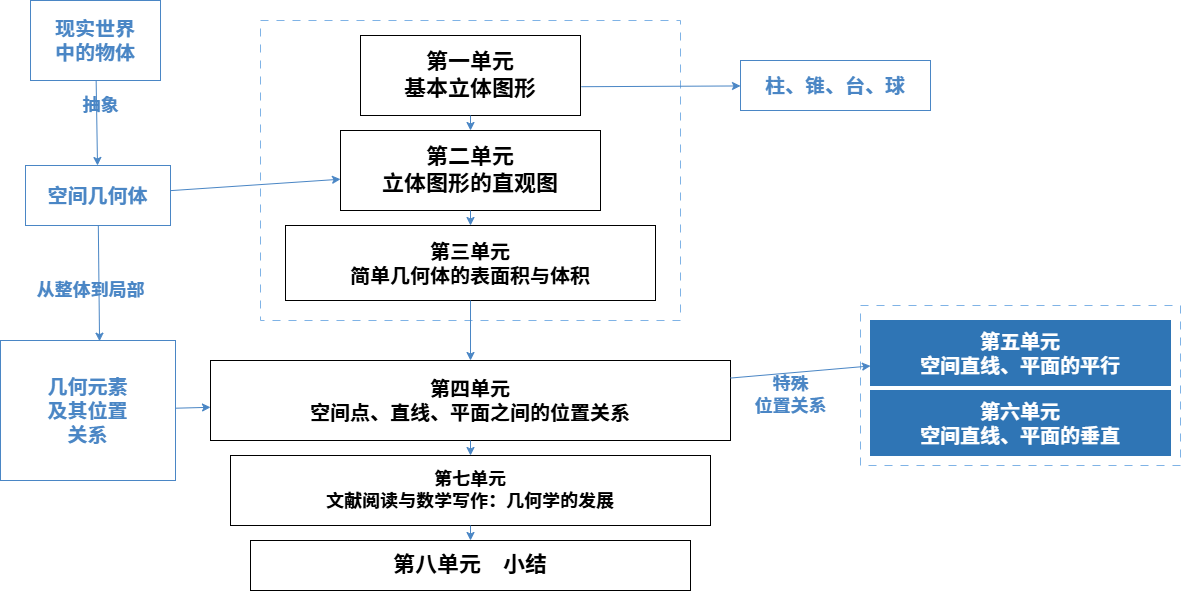
\includegraphics[width=1\textwidth]{../../image/单元内容/单元内容.png}
	\vspace{1em}
	\caption{立体几何初步单元内容结构图}
\end{figure}

\subsubsection{学情分析}

高一学生在进入"立体几何初步"学习之前，已经具备一定的平面几何知识基础，能够识别常见几何图形，理解部分基本概念，并能进行较为简单的几何推理。这为立体几何学习提供了必要的知识准备。然而，与平面几何相比，立体几何的研究对象由二维图形拓展到三维空间，学生需要在已有经验基础上完成思维方式的转换，这也是本单元学习中最容易出现困难的环节。

结合前文问卷调查分析可以看出，学生在立体几何学习中的主要问题集中体现在以下几个方面。首先，学生在二维图形与三维图形之间的转换能力较弱，尤其在观察直观图、还原空间结构和判断位置关系时容易出现偏差。其次，学生对空间中点、直线、平面之间关系的理解往往停留在直观判断层面，缺乏稳定的分析路径，导致在面对稍复杂的问题时难以准确作出推断。再次，在推理表达方面，学生常出现"能看图、难说理""有思路、难表述"的现象，即使能够凭借直觉作出判断，也难以用较为规范的数学语言说明其依据。

但与此同时，高一学生对模型操作、图形演示和问题探究具有较高的兴趣，愿意在具体情境中参与讨论和表达。这说明学生并非缺乏学习立体几何的积极性，而是需要更有效的教学支持。基于此，在本课设计中，应通过实物模型、图形表征、问题引导和交流反馈等方式为学生搭建学习支架，把抽象的空间关系转化为可观察、可操作、可表达的学习内容，帮助学生逐步建立空间观念，增强逻辑表达能力，并为后续更深入的立体几何学习奠定基础。

\subsubsection{目标分析}

基于前文的内容分析和学情分析，本单元目标设置主要依据两条线索：一是内容本身的知识逻辑，二是学生已有的学习起点。从内容结构看，"立体几何初步"呈现出由几何体直观认识到空间关系论证推理的递进过程，因此教学目标不能只停留在结论记忆，还应覆盖概念理解、关系刻画、定理应用和论证表达等层级。从学生实际看，高一学生在空间表象建构、二维与三维转换、数学语言表达方面仍较薄弱，但在模型操作和情境探究中参与意愿较强。基于这一现实，目标设计既要直面学生在"看图—判定—说理"链条中的关键困难，推动直观想象、逻辑推理与数学抽象能力逐步发展，也要保留问题情境和实践应用导向，提升学生将立体几何知识迁移到真实情境中的综合解决能力。

\begin{enumerate}
\item 数学抽象与逻辑推理素养：能够运用数学语言描述三维空间中的图形与关系，掌握立体几何的基本概念和性质，并能够通过逻辑推理证明相关命题。
\item 数学建模与问题解决素养：通过实际问题的引入和解决，培养学生运用立体几何知识建立数学模型的能力，以及运用这些模型解决实际问题的能力。同时，鼓励学生在解决问题的过程中进行探索和创新。
\item 数学运算与数据分析素养：进行适当的数学运算，如向量运算、角度计算等，提升他们的数学运算能力。同时，通过分析空间图形的数据特征，培养学生的数据分析能力。
\item 直观想象与空间观念素养：培养学生的空间观念，使他们能够想象并描述三维空间中的图形及其关系。鼓励学生运用直观想象来探究立体几何问题，提升他们的空间思维能力。
\item 数学文化与情感态度：了解数学在现实生活中的应用和价值，感受数学的魅力。同时，通过小组合作和探究学习，培养学生的团队合作精神和创新能力，使他们对数学学习保持积极的态度和浓厚的兴趣。
\end{enumerate}

\subsubsection{评价活动设计}

在"教学评一体化"理念下，《立体几何初步》单元的评价活动设计不应停留于对知识掌握结果的单一检测，而应立足核心素养发展，贯穿单元教学全过程。与其强调评价形式的多样化，不如更加关注评价是否真正指向学生素养的发展水平。因此，本单元评价活动设计应围绕直观想象、逻辑推理和数学抽象三项重点素养展开，通过持续收集学生在图形感知、关系判断、推理表达和综合应用中的学习证据，形成以素养发展为导向的单元评价体系。

具体而言，本单元可构建"感知与表征—分析与推理—抽象与应用"三层次素养评价体系。第一层次是感知与表征层，主要对应"基本立体图形""立体图形的直观图"等内容，重点评价学生是否能够识别常见空间几何体的结构特征，是否能够读懂直观图，是否能够在二维图形与三维图形之间进行基本的表征转换。第二层次是分析与推理层，主要对应"空间点、直线、平面之间的位置关系""空间直线、平面的平行与垂直"等内容，重点评价学生能否依据定义、判定和性质分析空间关系，能否在图形观察的基础上进行合理推断，并用较规范的数学语言完成说理和简单证明。第三层次是抽象与应用层，主要面向单元综合学习任务，重点评价学生是否能够把具体图形中的关系提升为一般性结论，并能够在综合问题和新情境中迁移运用所学知识，体现对单元内容的整体把握。

为了使上述评价目标真正落地，本单元需要选择具有针对性的评价工具。对于感知与表征层，可采用课堂观察表和学习任务单作为主要评价工具。教师在教学过程中可通过观察学生对模型、图形和直观图的辨识情况，记录其在空间想象和图形转换中的表现；同时，通过任务单中的识图、画图、判断等活动，收集学生对空间图形的感知和表征证据。对于分析与推理层，可采用板演展示记录、说理任务单和表现性评价量规，对学生在线面关系判断、判定定理运用、性质分析和推理表达中的表现进行评价，尤其关注其是否能够说明判断依据、是否能够用规范语言表达推理过程。对于抽象与应用层，则可采用单元综合任务单、学习反思单和综合测试题，考查学生能否将不同课时所学知识进行整合，并在新的问题情境中加以应用。

在实施路径上，本单元评价活动设计应形成"课前诊断—课中跟踪—课后反馈—单元总结"的闭环结构。课前可通过3—5道基础诊断题或简短学习单，了解学生对空间图形、基本位置关系和几何表达的已有基础，为教学起点的确定提供依据。课中则应依托课堂观察表、学习任务单、提问记录和板演展示，持续跟踪学生在模型观察、关系判断、推理说明和语言转化中的真实表现。例如在探究"直线与平面平行"相关问题时，不仅要关注学生是否能作出正确判断，还要关注其是否在文字语言、数学语言、符号语言之间进行有效转化。通过这种多样化的评价方式，教师能够及时发现学生在理解和表达方面的困难，并通过调整教学策略、提供针对性指导来促进学生的思维发展和素养提升。同时，这种过程性评价也有助于激发学生的学习兴趣和参与度，使其在积极参与中不断完善对空间关系的理解。课后可通过分层练习、错题反思单、自评互评表等方式，引导学生总结自己在图形理解、关系判断和推理表达中的主要问题。单元结束后，可通过综合测试、单元表现性任务或综合性说理题，对学生在整个单元中的素养发展情况作整体判断。

\begin{figure}[H]
	\centering

	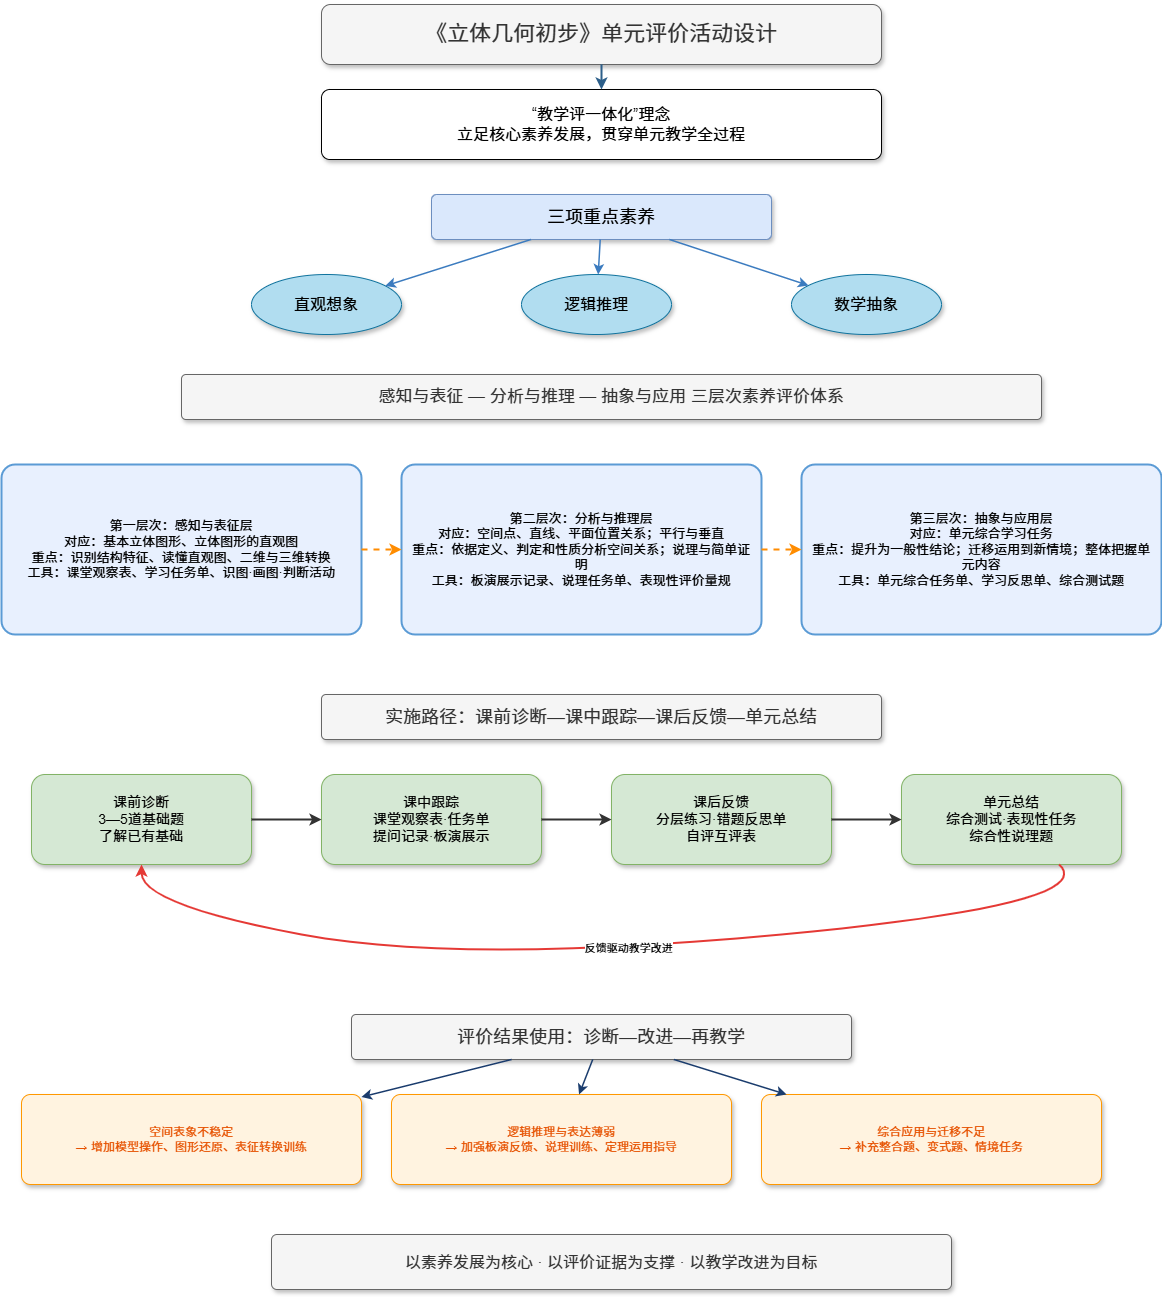
\includegraphics[width=1\textwidth]{../../image/评价设计/评价.png}
	\vspace{1em}
	\caption{评价设计}
\end{figure}
为增强评价活动的可操作性，本单元还应明确评价结果的使用方式。若学生在"基本立体图形"或"直观图"相关内容中错误较多，说明其空间表象尚不稳定，教师应增加模型操作、图形还原和表征转换训练；若学生在线面平行、线面垂直等内容中判断失误较多，或虽然能得出结论却无法说明依据，说明其逻辑推理和数学表达能力仍较薄弱，教师应加强板演反馈、说理训练和定理运用指导；若学生在单元综合任务中表现出知识迁移不足、综合应用能力较弱，则应补充单元整合题、变式题和情境任务，引导学生从零散知识走向结构化理解。通过这种以素养发展为核心、以评价证据为支撑、以教学改进为目标的单元评价活动设计，可以更好地发挥评价的诊断、反馈和促进功能，从而提升《立体几何初步》单元教学的整体质量。

\subsection{《直线与平面平行》课时设计}

此课时内容处于空间位置关系学习的重要节点，既承接前面关于空间点、直线、平面的初步认识，又为后续学习线面垂直、面面平行、面面垂直以及立体几何证明打下基础。从知识价值来看，本课是学生认识线面关系、理解空间平行关系的重要起点；从思维价值来看，本课需要学生在图形观察的基础上对空间关系作出判断，并进一步尝试用数学语言说明判断依据，这对于促进学生由直观感知走向逻辑表达具有重要意义。因此，将本课作为案例内容，不仅具有较强的代表性，也有利于呈现立体几何教学中核心素养落实的关键环节。

\subsubsection{《直线与平面平行》教学目标与核心素养对应表}

\renewcommand\arraystretch{1.5}
\begin{longtable}{|>{\centering\arraybackslash}p{0.47\textwidth}|>{\centering\arraybackslash}p{0.12\textwidth}|>{\centering\arraybackslash}p{0.27\textwidth}|}
\caption{\label{tab4.1}《直线与平面平行》教学目标与数学学科核心素养对应.} \\
\hline
教学目标 & 对应核心素养 & 具体体现 \\
\hline
能从直线与平面平行的定义出发，借助长方体等，猜想直线与平面平行的充分条件，并通过具体实例进行验证，归纳出直线与平面平行的判定定理。 & 直观想象 & 学生借助长方体等空间模型观察线面位置关系，形成空间表象，并在图形感知中理解线面平行的几何意义。 \\
\hline
能从直线与平面平行的定义出发，借助长方体等，猜想直线与平面平行的充分条件，并通过具体实例进行验证，归纳出直线与平面平行的判定定理。 & 逻辑推理 & 学生经历"观察—猜想—验证—归纳"的过程，在已有定义基础上推导判定条件，体现了推理论证能力的发展。 \\
\hline
能用自己的语言解释直线与平面平行的判定定理，并能用三种语言进行准确描述。 & 数学抽象 & 学生将具体图形中的位置关系概括为一般性的数学结论，实现由具体实例到抽象定理的提升。 \\
\hline
会用定义和判定定理判定直线与平面平行。 & 逻辑推理 & 学生能够依据已知条件调用定义和定理，对线面关系作出合理判断，体现演绎推理意识。 \\
\hline
能在明确直线与平面平行的性质所研究的问题的基础上，以直线与平面平行为条件，分析直线与平面内直线的位置关系，得出直线与平面平行性质的猜想，并能用三种语言描述。 & 逻辑推理 & 学生在条件分析、关系推断和性质猜想中逐步形成较完整的推理链条，体现逻辑推理素养。 \\
\hline
能在明确直线与平面平行的性质所研究的问题的基础上，以直线与平面平行为条件，分析直线与平面内直线的位置关系，得出直线与平面平行性质的猜想，并能用三种语言描述。 & 直观想象 & 学生需要借助空间图形想象线与面、线与线之间的位置变化，在图形表征中理解性质成立的条件。 \\
\hline
能证明猜想得出直线与平面平行的性质；能用自己的语言解释直线与平面平行的性质定理。 & 数学抽象 & 学生能够将图形关系上升为一般性的性质结论，并用较为概括的数学语言进行解释和表述。 \\
\hline
能用直线与平面平行的性质定理解决简单问题。 & 数学运算 & 在简单问题解决过程中，学生需要结合定理进行关系判断和推演，体现一定的数学运算与处理能力。 \\
\hline
\end{longtable}

\vspace*{-10pt}

从总体上看，本课教学目标主要指向直观想象、逻辑推理和数学抽象三项核心素养，其中以直观想象和逻辑推理最为突出；数学建模与数据分析在本课中体现较弱，不作为本课重点素养目标。

\subsubsection{教学重难点}

\textbf{教学重点}：直线与平面平行的判定定理、性质定理。

\textbf{教学难点}：直线与平面平行的判定定理、性质定理的发现过程，及其应用。

\subsubsection{教学过程}

\begin{enumerate}
    \item \textbf{观察实验，归纳定理}

\begin{itemize}
    \item \textbf{问题1}

门扇的两边是平行的，当门扇绕着一边转动时，另一边与墙面有公共点吗？此时门扇转动的一边与墙面平行吗？观察实验，将门扇的边看成直线，墙面看成平面，你能得到什么猜想？

\textbf{师生活动}

学生依次观察两个实验，作出猜想。学生观察门扇，并思考，因为对边互相平行，没有交点，因此门扇不论转动到什么位置，它能活动的竖直的一边始终与固定的竖直一边没有交点，与墙面也没有交点，根据定义，猜想它们之间是平行的。

    \item \textbf{追问1}

如上归纳出来的就是直线与平面平行的判定定理，如何用三种语言表示？阅读教科书第136页，给出回答。

\textbf{师生活动}

学生阅读教科书，获得准确的三种语言表述。

（1）文字语言：直线与平面平行的判定定理——如果平面外一条直线与此平面内的一条直线平行，那么该直线与此平面平行。

（2）图形表示：可以有多种表示方法，其中之一如图8.5-9所示。

（3）符号表示：$a\not\subset A$，$b\subset A$，且$a\parallel b\Rightarrow a\parallel A$。

    \item \textbf{追问2}

去掉判定定理中的条件$a\not\subset A$，直线$a$与平面$A$的位置关系是什么？写出结论。据此，在应用判定定理时应该注意什么？可以结合两个实验中的模型进行分析。

\textbf{师生活动}

学生依据直线$a$与平面$A$的位置关系分类讨论求解。若去掉条件$a\not\subset A$，那么直线$a$与平面$A$的位置关系有两种：$a\subset A$与$a\parallel A$。所以，得到的结论是：$b\subset A$，且$a\parallel b\Rightarrow a\parallel A$或$a\subset A$。因此在利用判定定理解决问题时，要注意条件完备，缺一不可。

    \item \textbf{追问3}

依据直线与平面平行的判定定理判定直线与平面平行的思路是什么？直线与平面平行的判定定理的本质是什么？

\textbf{师生活动}

学生可以得出思路是直线与平面平行问题转化为直线与直线平行问题，判定定理本质上反映了直线与平面的组成元素（把平面看成是由直线组成的）之间特定的位置关系。

    \item \textbf{追问4}

这一定理在现实生活中有许多应用。例如，安装矩形镜子时，为了使镜子的上边框与天花板平行，可以先在天花板上画一条水平线，再让镜子的上边框与这条水平线平行。你能想到其他的应用吗？请举例说明。

\textbf{师生活动}

学生依据直线与平面平行的判定定理可以解决。举例略。
\end{itemize}

\textbf{设计意图}

结合实例，通过直观感知与操作验证，引导学生归纳直线与平面平行的判定定理。在此过程中，教师进一步引导学生认识到：研究直线与平面的位置关系，可以转化为研究该直线与构成平面的几何要素（即平面内直线）的位置关系，从而渗透"转化研究"的一般观念，培养学生的数学探究能力。随后，通过阅读教材，学生学习并掌握该定理的三种规范表达。追问2通过变式设计，引导学生从反面审视判定定理，进而形成严谨的思维习惯；同时帮助学生理解定理的本质，以及运用定理解题的基本思路。最后，将定理应用于实际问题的解决，使学生体会数学与生活的紧密联系，感受数学的应用价值。

\textbf{评价活动}

\renewcommand\arraystretch{1.5}
\begin{longtable}{|>{\centering\arraybackslash}p{0.10\textwidth}|>{\centering\arraybackslash}p{0.26\textwidth}|>{\centering\arraybackslash}p{0.15\textwidth}|>{\centering\arraybackslash}p{0.34\textwidth}|}
\caption{\label{tab4.2}观察实验、归纳定理环节评价活动.} \\
\hline
评价内容 & 评价任务 & 评价方式 & 目标达成依据（四级）\\
\hline
直观观察与问题提出 & 基于"门扇转动"情境，判断活动边与墙面是否有公共点，并提出"何时可判定线面平行"的初步猜想。 & 教师提问与追问、学生口头回答、同伴补充 & 优：能准确判断并主动提出有依据的猜想；良：能正确判断并在提示下形成猜想；中：能部分判断但猜想不完整；待改进：判断与猜想均较模糊。 \\
\hline
判定条件归纳 & 从定义出发，归纳"线面平行判定定理"的关键条件，并说明条件缺失可能导致的结果变化。 & 小组讨论、板演展示、教师点拨 & 优：能完整归纳条件并清晰说明"条件完备性"；良：能归纳主要条件，解释基本正确；中：能说出部分条件但逻辑不连贯；待改进：条件识别不清，难以解释。 \\
\hline
定理表述与规范表达 & 将判定定理转化为规范数学表述（文字叙述与符号表达），并做到前提、结论对应清楚。 & 课堂练写、投影讲评、互评修正 & 优：表述规范、符号准确、逻辑对应完整；良：表述基本正确，个别符号或逻辑细节欠严谨；中：表述有明显缺漏但核心意思可辨；待改进：表述混乱，前提结论对应错误。 \\
\hline
变式辨析与错误诊断 & 对"去掉某条件后是否仍可判定线面平行"等变式进行辨析，指出常见误判原因。 & 变式练习、即时反馈、错因讨论 & 优：能独立完成辨析并准确定位错因；良：能完成多数辨析并在提示下说明错因；中：能判断部分题目但错因说明笼统；待改进：辨析困难，错因不清。 \\
\hline
迁移应用与反思 & 在简单新情境中应用判定定理完成判断，并用简短反思说明"本节最关键的判定思路"。 & 当堂小测、学生自评、教师点评 & 优：迁移应用准确，反思能概括"线面问题转化为线线问题"的核心思路；良：应用基本正确，反思较清晰；中：应用有误但能说出部分思路；待改进：应用与反思均较薄弱。 \\
\hline
\end{longtable}


    \item \textbf{逆向思考，归纳性质}

\begin{itemize}
    \item \textbf{问题2}

我们利用平面内的直线与平面外的直线平行，得到了判定平面外的直线与此平面平行的方法，即得到了一条直线与平面平行的充分条件。反过来，如果一条直线与一个平面平行，能推出哪些结论呢？这就是要研究直线与平面平行的性质，也就是研究直线与平面平行的必要条件。

    \item \textbf{追问1}

直线与平面平行的判定定理本质上是通过平面外一条直线与平面内直线的平行关系判定平面外的直线与此平面平行。按照这样的思路，反过来，已知$a\parallel\alpha$，直线$a$与平面$\alpha$内的直线有怎样的位置关系呢？请仿照判定定理的探究过程，用笔代表直线，桌面代表平面，操作演示，观察现象，作出判断。

\textbf{师生活动}

学生利用笔和桌面做实验，直观感知，操作确认：笔与桌面平行，即笔与桌面没有公共点，所以笔与桌面内的直线没有公共点，即笔与桌面内的直线有平行、异面两种情况。进而归纳出结论：与平面平行的直线与此平面内的直线的位置关系有平行、异面两种情况。

    \item \textbf{追问2}

已知$a\parallel\alpha$，你能利用两条直线相互平行的定义，在平面$\alpha$内找出一条与直线$a$平行的直线$b$吗？

\textbf{师生活动}

学生独立思考后小组讨论，再进行全班交流，教师引导学生得出：因为两条直线相互平行的定义是"同一平面内的两条没有公共点的直线叫做平行线"，所以，设直线$a$所在的平面为$\beta$，$\beta$与$\alpha$的交线为$b$，如果直线$b$与直线$a$没有公共点，那么它们就相互平行，这是显然的。因为如果$a$与$b$有公共点的话，$a$就与$\alpha$有公共点，这与$a\parallel\alpha$矛盾。由此，不仅得出了猜想，而且也从形成猜想的过程中得到了证明猜想的思路——反证法。

    \item \textbf{追问3}

你能证明上述猜想吗？已知是什么？结论是什么？

\textbf{师生活动}

学生依据追问2中的分析过程获得证明思路，独立完成之后展示交流。

已知：$a\parallel\alpha$，$a\subset\beta$，$\alpha\cap\beta=b$。

求证：$a\parallel b$。

证明：$\because\alpha\cap\beta=b$，$\therefore b\subset\alpha$。

又$a\parallel\alpha$，$\therefore a$与$b$没有公共点。

又：$a\subset\beta$，$b\subset\beta$。

$\therefore a\parallel b$。

    \item \textbf{追问4}

关于直线与平面平行的性质定理，你能用三种语言表示它吗？请你阅读教科书137页完成。

\textbf{师生活动}

学生自主完成。

（1）文字语言：一条直线与一个平面平行，如果过该直线的平面与此平面相交，那么该直线与交线平行。

（2）图形表示：如图所示。

（3）符号表示：$a\parallel\alpha$，$a\subset\beta$，$\alpha\cap\beta=b$，$\therefore a\parallel b$。

    \item \textbf{追问5}

直线与平面平行的性质定理的本质是什么？作用是什么？

\textbf{师生活动}

学生类比判定定理可以得出结论。本质是由直线与平面平行推导出直线与直线平行，可以用于证明线线平行。
\end{itemize}

\textbf{设计意图}

通过创设问题情境，引导学生沿着数学知识内部发展的逻辑展开探究。追问1通过类比问题1，在一般观念的引导下开展实验探究；追问2在追问1的基础上，进一步探讨如何通过条件强化获得确定性结论，并据此形成猜想；后续三个追问则引导学生完成三种语言的规范表达与严谨论证，进而理解定理的本质及其作用。通过这一过程，学生依次经历直观感知、操作确认、提出猜想与严谨论证，逐步提升在一般观念指导下开展数学探究的能力。

\textbf{评价活动}

\renewcommand\arraystretch{1.5}
\begin{longtable}{|>{\centering\arraybackslash}p{0.10\textwidth}|>{\centering\arraybackslash}p{0.26\textwidth}|>{\centering\arraybackslash}p{0.15\textwidth}|>{\centering\arraybackslash}p{0.34\textwidth}|}
\caption{\label{tab4.3}逆向思考、归纳性质环节评价活动.} \\
\hline
评价内容 & 评价任务 & 评价方式 & 目标达成情况 \\
\hline
逆向思考与性质意识 & 围绕"由判定反推性质"这一问题，判断学生能否从已有判定定理自然过渡到对性质定理的探究，初步形成逆向思考意识。 & 教师提问、学生口头回答、同伴补充 & 优：能主动从判定联想到性质，明确本节研究的是必要条件；良：能在教师提示下理解由判定转向性质的研究思路；中：只能重复问题情境，尚不能准确说出探究方向。 \\
\hline
直观操作与关系判断 & 借助"笔—桌面"模型操作，判断学生能否通过观察和操作发现"与平面平行的直线与平面内直线有平行、异面两种位置关系"。 & 模型操作、课堂观察、口头汇报 & 优：能准确操作并概括出平行、异面两种情况，说明判断依据；良：能通过操作得出正确结论，但表述不够完整；中：只能进行直观判断，不能清楚说明位置关系。 \\
\hline
构造辅助线与形成猜想 & 在已知$a\parallel\alpha$的条件下，判断学生能否在平面$\alpha$内构造出与$a$平行的直线$b$，并说明构造依据。 & 独立思考、小组讨论、全班交流 & 优：能准确构造交线$b$，并从"同一平面内且无公共点"说明$a\parallel b$；良：能在讨论后完成构造，但理由表达不够严密；中：能够接受构造结果，但不能独立说明构造思路。 \\
\hline
证明过程与推理表达 & 根据追问2形成的思路，判断学生能否明确已知、求证，并完成性质定理的规范证明。 & 板演展示、教师点评、学习单记录 & 优：已知、求证清晰，证明步骤完整，逻辑严密；良：能完成主要证明过程，但部分依据表达不够规范；中：能写出部分步骤，但前提、结论或推理链条不完整。 \\
\hline
三种语言转化 & 判断学生能否用文字语言、图形语言和符号语言准确表述直线与平面平行的性质定理。 & 自主填写、同伴互查、教师核对 & 优：三种语言表述准确、对应关系清晰；良：基本能够完成三种表述，但符号或文字表达存在个别疏漏；中：只能完成其中一到两种表述，语言转化不够准确。 \\
\hline
性质本质与作用理解 & 围绕"性质定理的本质和作用是什么"展开评价，判断学生能否认识到该定理的核心是"线面平行转化为线线平行"，并理解其在后续证明中的作用。 & 课堂追问、学生归纳、教师总结 & 优：能准确概括性质本质，并说明其在推理和解题中的转化作用；良：能说出"转化"这一关键点，但作用分析不够深入；中：只能复述定理内容，尚不能概括其本质与功能。 \\
\hline
\end{longtable}

\vspace*{-10pt}

\end{enumerate}

\section{结语}

\subsection{研究结论}

本研究聚焦高中数学“立体几何初步”单元，结合课程标准分析、教师问卷调查与课例建构，形成了两类结论：一是观点层面的认识推进，二是实践层面的实施方案。

在观点层面，本文提出五点主张。第一，教学评一体化在立体几何单元中的推进，重点不应停留在理念阐释，而应落到可操作设计上。也就是说，素养目标必须转化为课时中可观察、可评价、可实施的学习行为。第二，直观想象、逻辑推理与数学抽象不宜分割处理，更适合在同一任务链中协同发展。第三，单元组织方式应由“知识点顺排”逐步转向“核心问题或大概念统领”，通过问题链统摄课时活动与评价任务。第四，评价在立体几何教学中不只是结果判定工具，更应承担过程调控功能，直接服务教学决策和学习改进。第五，必修阶段需要守住综合法推理训练的基础地位，再与选修阶段的向量方法形成有层次的衔接，避免“方法替代思维”。

在措施层面，本文形成四项可执行方案。第一，提出“素养目标-课时任务-评价指标”三级转化路径，把抽象目标落细到课堂活动与证据采集。第二，构建“课前诊断-课中跟踪-课后反馈”的评价闭环，使评价前置、过程伴随、结果回用。第三，围绕《立体几何初步》单元与《直线与平面平行》课时，示范“目标-活动-评价”一致性的设计方式，提供可复用范式。第四，提出“校本教研共建+高校中学协同”的推进机制，将案例供给、量规开发、同伴互助和专题培训纳入常态化支持。

这些结论与措施具有较强现实针对性。调查显示，教师对单元整体设计认同度较高，对评价工具、课时案例和模板资源的需求也更为集中。在这一背景下，本文提出的方案并非概念堆叠，而是对一线真实问题的结构化回应。其关键意义在于，把“教什么、怎么教、如何评、怎样改”放进同一逻辑链条，推动教学评一体化由零散尝试走向系统实施。

综上，本文并不止于描述问题，而是提出并论证了一套可迁移、可改编、可持续优化的立体几何单元教学评一体化方案。该方案以单元整体设计为框架，以评价闭环为运行机制，以案例化工具为落地抓手，为核心素养导向的课堂改进提供了可执行路径。

\subsection{研究启示}

基于上述结论，本文提出以下实践启示。

其一，在教学设计层面，素养目标的课时化与任务化应成为起点工作。教师需要先界定学生在直观想象、逻辑推理、数学抽象上的可观察表现，再倒推学习任务与评价任务。与“先讲后测”的惯性路径相比，这种逆向设计更能避免目标与评价脱节，也更便于课堂中的即时诊断与动态调整。

其二，在课堂实施层面，需要从“演示主导”走向“建构参与”。立体几何确实依赖图形感知，但仅靠教师展示，学生很难形成稳定空间观念。课堂可适度增加模型操作、图形互化、同伴解释、板演说理等活动，让学生在“观察-表达-论证-修正”的循环中真正完成知识建构。对“能判断却说不清”的学生，结构化说理模板与分层反馈尤其有效。

其三，在评价改进层面，应形成覆盖课前、课中、课后的三层系统。课前用简短诊断明确学习起点，课中用提问、观察、任务单和即时反馈跟踪过程，课后通过分层练习、反思单与综合任务检验迁移。评价工具的价值不在“记录分数”，而在“支持决策”。立体几何单元可优先开发简明量规，提升日常课堂中的可用性。

其四，在教研组织层面，资源共建与专业互助应成为推进重点。调查反复显示，一线教师最需要的是可参照、可改编、可直接上手的案例与模板。学校与教研组可围绕同一单元建立“共备-共研-共评”机制，积累本校可复用的任务库和量规样例。同时，应加强与高校、区域教研机构协作，把理论成果转化为课堂方案，缩短“知道”到“做到”的距离。

其五，在课程实施层面，应坚持必修阶段综合法训练的基础地位，并稳妥处理与向量法的衔接。教师普遍反馈，向量法在某些教学情境下会压缩综合法训练空间。因此，必修阶段应优先保障空间关系的直观分析与综合说理，选修阶段再逐步强化向量工具应用，并通过“一题多解”培养方法选择能力。方法可以多元，但思维训练不能被替代。

总体而言，这些启示可归结为一句话：教学评一体化不是简单加环节，而是重构教学流程。它要求教师把“教什么、怎么教、怎么评、如何改”放在同一框架中持续运作，由此提升立体几何单元教学的针对性、连贯性与育人实效。

\subsection{反思与展望}

本研究在立体几何单元教学评一体化的理论梳理、现状调查与案例建构方面做了系统尝试，但仍有改进空间。

首先，样本覆盖面与区域代表性仍可拓展。不同地区、不同学校类型在课程资源、技术条件和教研支持上差异明显，这会直接影响教学评一体化的实施强度。后续研究可扩大样本规模，开展跨区域比较，以提升结论的普遍解释力。

其次，研究范围主要聚焦必修阶段“立体几何初步”单元，对选修阶段向量方法主导情境下的一体化设计讨论仍不充分。未来可围绕必修与选修衔接，进一步研究“综合法-向量法协同”框架下的目标设置、任务组织与评价标准，形成更完整的学段化路径。

再次，效果验证仍需长期证据。本文提出的设计思路主要依据调查材料与案例论证，尚缺少大样本、长周期的实证跟踪。后续可结合课堂实验与学习过程数据，持续观察其对空间观念、推理表达和迁移应用的影响，增强研究结论的外部效度。

最后，教育数字化为过程性评价提供了新机会，也带来新风险。未来可探索信息技术支持下的学习证据采集、可视化反馈和数据应用机制，但前提必须明确：技术服务教学改进，而不是替代教学目标。

总体来看，本研究的价值在于给出一个可执行方向：以单元整体设计为载体，把核心素养目标、学习活动与评价反馈整合为可循环的教学系统。下一步工作将继续围绕“证据驱动的课堂改进”推进，使教学评一体化在立体几何教学中从阶段性实践走向常态化机制。

\newpage
%正文结束

%参考文献
\begin{thebibliography}{99}
\addcontentsline{toc}{section}{\protect 参考文献}
\setlength{\itemsep}{-0.75ex}
%请把文献条目填写在下面,例如
\bibitem{xiao2025}肖诗刚.``教-学-评''一体化视域下的高中数学教学策略[J].中小学班主任,2025(24):48-50.
\bibitem{zhao2024}赵德成.``教-学-评''一致性何以可能[J].课程,2024,44(5):55-63.
\bibitem{zhang2020}章建跃.数学学科核心素养导向的``单元-课时''教学设计[J].中学数学教学参考,2020(13):5-12.
\bibitem{zhao_ping2022}赵萍,郭泽琳.深度学习视域下逆向单元教学设计在高中数学教学中的应用成效[J].华南师范大学学报(社会科学版),2022(3):54-65+206.
\bibitem{lai2024}赖婷婷.核心素养背景下高中数学课堂``教、学、评''一致性研究:以函数的概念与性质为例[D].广西民族大学,2024.
\bibitem{xu2017}徐敏标.高中数学``教、学、评''一致性研究的总体路径与思考[J].教育研究与评论(中学教育教学),2017(6):8-13.
\bibitem{shi2017}史宁中.高中数学核心素养的培养、评价与教学实施[J].中小学教材教学,2017(5):4-9.
\bibitem{cui_lei2015}崔允漷,雷浩.教-学-评一致性三因素理论模型的建构[J].华东师范大学学报(教育科学版),2015,33(4):15-22.
\bibitem{li2019}李海东.基于核心素养的``立体几何初步''教材设计与教学思考[J].数学教育学报,2019,28(1):8-11.
\bibitem{lei2023}雷浩.基于核心素养的``教-学-评''一致性探讨[J].课程,2023,43(10):42-49.
\bibitem{wang2012}王超.新课程理念下高中立体几何教学的研究与实践[D].华中师范大学,2012.
\bibitem{zhang2016}章建跃.高中数学教材落实核心素养的几点思考[J].课程,2016,36(7):44-49.
\bibitem{zhu2018}朱立明,胡洪强,马云鹏.数学核心素养的理解与生成路径:以高中数学课程为例[J].数学教育学报,2018,27(1):42-46.
\bibitem{pan2025}潘燚云.基于核心素养的高中数学单元教学设计:以``基本立体图形''为例[J].新课程,2025(35).
\bibitem{ke2025}柯惠芬.范希尔理论下高一学生立体几何学习障碍的调查研究:以昆明市S中学为例[D].云南师范大学,2025.
\bibitem{fan2025}范祖库.基于``教-学-评''一体化的高中数学逆向教学设计探究:以《圆锥曲线的方程》章起始课为例[J].教学月刊-中学版(教学参考),2025.
\bibitem{cui_xia2013}崔允漷,夏雪梅."教-学-评一致性":意义与含义[J].中小学管理,2013(1):4-6.
\bibitem{gaozhong_kebiao}中华人民共和国教育部.普通高中数学课程标准(2017年版2025年修订)[S].北京:人民教育出版社,2020.
\bibitem{Black}Black P, Wiliam D. Assessment and Classroom Learning[J]. Assessment in Education: Principles, Policy \& Practice, 1998, 5(1): 7-74.
\bibitem{schenck}Schenck K E, Nathan M J. Navigating Spatial Ability for Mathematics Education: a Review and Roadmap[J]. Educational Psychology Review, 2024, 36(3): 90
\end{thebibliography}
\newpage
\section*{\centerline{致\quad 谢}}
\addcontentsline{toc}{section}{\protect 致谢}
感谢!
\newpage
\section*{\centerline{附\quad 录}}
\addcontentsline{toc}{section}{\protect 附录}

\subsection*{指向核心素养的高中数学“立体几何”单元教学评一体化调查问卷}

尊敬的老师：

您好！为了解当前高中数学“立体几何”单元教学中教学评一体化的实施现状、核心素养落实情况、评价方式与工具使用情况，以及教师对后续教学优化的需求，特开展本次问卷调查。问卷采用匿名方式，调查结果仅用于研究分析，请您结合实际教学情况如实填写。

衷心感谢您的支持与配合！

\subsection*{一、基本信息}

\subsubsection*{1.您的性别}
\begin{itemize}
\item □男
\item □女
\end{itemize}

\subsubsection*{2.您的教龄}
\begin{itemize}
\item □5年以下
\item □5—10年
\item □11—15年
\item □16—20年
\item □20年以上
\end{itemize}

\subsubsection*{3.您任教学校的类型}
\begin{itemize}
\item □省级示范性高中
\item □市级重点高中
\item □普通高中
\item □其他
\end{itemize}

\subsubsection*{4.您目前任教的年级}
\begin{itemize}
\item □高一
\item □高二
\item □高三
\item □跨年级任教
\end{itemize}

\subsubsection*{5.您是否长期承担立体几何相关内容教学}
\begin{itemize}
\item □是
\item □否
\end{itemize}

\subsection*{二、教师对“教学评一体化”理念的认知与实践现状}

\subsubsection*{6.您对“教学评一体化”理念的了解程度是}
\begin{itemize}
\item □非常了解
\item □比较了解
\item □听说过但了解不多
\item □基本不了解
\end{itemize}

\subsubsection*{7.您认为“教学评一体化”的核心内涵包括}
（可多选）
\begin{itemize}
\item □教学目标、学习活动与评价标准保持一致
\item □评价贯穿教学全过程
\item □根据评价结果及时调整教学
\item □评价兼顾学习过程与学习结果
\item □其他：\underline{\hspace{2cm}}
\end{itemize}

\subsubsection*{8.您在立体几何教学中落实“教学评一体化”的总体情况是}
\begin{itemize}
\item □经常系统实施
\item □偶尔实施
\item □有意识尝试但不够系统
\item □很少实施
\item □从未实施
\end{itemize}

\subsubsection*{9.您在立体几何教学中使用过哪些过程性评价方式}
（可多选）
\begin{itemize}
\item □课堂提问
\item □随堂练习
\item □学习单
\item □课堂观察记录
\item □学生自评/互评
\item □表现性任务
\item □其他：\underline{\hspace{2cm}}
\end{itemize}

\subsubsection*{10.您认为推进立体几何单元教学评一体化的主要困难是}
（可多选）
\begin{itemize}
\item □课时紧张
\item □缺少单元案例
\item □缺少评价工具或量规
\item □素养目标不易转化为具体任务
\item □信息技术支持不足
\item □教师培训不够
\item □其他：\underline{\hspace{2cm}}
\end{itemize}

\subsection*{三、立体几何单元教学中核心素养的落实情况}

\subsubsection*{（一）直观想象素养的培养}

\subsubsection*{11.您认为立体几何单元对培养学生直观想象素养的作用是}
\begin{itemize}
\item □非常重要
\item □比较重要
\item □一般
\item □不太重要
\item □不重要
\end{itemize}

\subsubsection*{12.您在教学中通常使用哪些方式帮助学生形成空间直观}
（可多选）
\begin{itemize}
\item □实物模型
\item □教师示意图
\item □多媒体课件
\item □动态几何软件
\item □学生活动操作
\item □生活情境引入
\item □其他：\underline{\hspace{2cm}}
\end{itemize}

\subsubsection*{13.您认为学生在立体几何学习中最常见的困难是}
（可多选）
\begin{itemize}
\item □二维图形与三维图形转化困难
\item □三视图与直观图互化困难
\item □空间位置关系判断困难
\item □空间想象不稳定
\item □其他：\underline{\hspace{2cm}}
\end{itemize}

\subsubsection*{14.您认为信息技术手段对培养学生直观想象素养的帮助程度是}
\begin{itemize}
\item □非常大
\item □比较大
\item □一般
\item □不太大
\item □基本没有作用
\end{itemize}

\subsubsection*{（二）逻辑推理素养的培养}

\subsubsection*{15.您认为立体几何证明题对培养学生逻辑推理素养的作用是}
\begin{itemize}
\item □非常明显
\item □比较明显
\item □一般
\item □不太明显
\item □不明显
\end{itemize}

\subsubsection*{16.学生在立体几何推理表达中常见的问题有}
（可多选）
\begin{itemize}
\item □推理链条不完整
\item □证明步骤跳跃
\item □符号使用不规范
\item □因果关系表述不清
\item □不会结合图形组织证明思路
\item □其他：\underline{\hspace{2cm}}
\end{itemize}

\subsubsection*{17.您在教学中是否会设计“一题多解”（综合法与向量法对比）活动}
\begin{itemize}
\item □经常
\item □偶尔
\item □很少
\item □从不
\end{itemize}

\subsubsection*{（三）数学抽象及其他素养的渗透}

\subsubsection*{18.您认为立体几何教学中“数学抽象”素养的呈现程度是}
\begin{itemize}
\item □非常明显
\item □比较明显
\item □一般
\item □不太明显
\item □很不明显
\end{itemize}

\subsubsection*{19.您在立体几何单元中是否会设计与数学建模或真实情境相关的活动}
\begin{itemize}
\item □经常
\item □偶尔
\item □很少
\item □从不
\end{itemize}

\subsubsection*{20.您认为影响核心素养目标在立体几何课时中落实的主要原因是}
（可多选）
\begin{itemize}
\item □目标表述较抽象
\item □缺乏与课时对应的任务设计
\item □缺乏配套评价工具
\item □教学时间不足
\item □学生差异较大
\item □其他：\underline{\hspace{2cm}}
\end{itemize}

\subsection*{四、立体几何单元教学的评价方式与评价工具现状}

\subsubsection*{21.您在立体几何单元中最常用的评价方式是}
（可多选）
\begin{itemize}
\item □课堂练习
\item □单元测试
\item □作业评价
\item □课堂观察
\item □学生自评/互评
\item □表现性任务
\item □学习档案袋
\item □其他：\underline{\hspace{2cm}}
\end{itemize}

\subsubsection*{22.您是否使用过评分量规（rubric）评价学生在立体几何学习中的表现}
\begin{itemize}
\item □经常使用
\item □偶尔使用
\item □听说过但未使用
\item □从未使用
\end{itemize}

\subsubsection*{23.您在设计评价任务时，是否会系统对照教学目标}
\begin{itemize}
\item □每次都会
\item □经常会
\item □偶尔会
\item □很少会
\item □从不会
\end{itemize}

\subsubsection*{24.您是否会依据评价结果及时调整后续立体几何教学}
\begin{itemize}
\item □经常会
\item □偶尔会
\item □很少会
\item □从不会
\end{itemize}

\subsection*{五、立体几何单元教学评一体化设计的需求与建议}

\subsubsection*{25.您是否认同“以单元为单位进行设计更有利于核心素养落实”}
\begin{itemize}
\item □非常认同
\item □比较认同
\item □一般
\item □不太认同
\item □不认同
\end{itemize}

\subsubsection*{26.您最希望获得哪类单元教学支持资源}
（可多选）
\begin{itemize}
\item □单元整体教学案例
\item □目标—活动—评价一致性设计模板
\item □核心问题链设计示例
\item □课时任务设计案例
\item □情境化教学素材
\item □其他：\underline{\hspace{2cm}}
\end{itemize}

\subsubsection*{27.您最希望获得哪类评价与支持资源}
（可多选）
\begin{itemize}
\item □直观想象素养评价量规
\item □逻辑推理素养评价量规
\item □表现性任务设计模板
\item □课堂观察量表或学习单示例
\item □信息化评价平台支持
\item □高校—中学协同教研或专题培训
\item □其他：\underline{\hspace{2cm}}
\end{itemize}

\subsection*{六、开放性问题}

\subsubsection*{28.您认为当前高中立体几何教学中最值得改进的一个方面是什么？}

\subsubsection*{29.您在立体几何教学中有哪些较成功的教学评一体化实践经验？}

\subsubsection*{30.您对后续优化高中立体几何单元教学评一体化设计还有哪些建议？}

\end{document}






